%%%%%%%%%%%%%%%%%%%%%%%%%%%%%%%%%%%%%%%%%%  不使用 authblk 包制作标题  %%%%%%%%%%%%%%%%%%%%%%%%%%%%%%%%%%%%%%%%%%%%%%
%-------------------------------PPT Title-------------------------------------
\title{赝势理论在第一原理计算方法中的地位}
%-----------------------------------------------------------------------------

%----------------------------Author & Date------------------------------------
\author[\textrm{Jun\_Jiang}]{姜\;\;骏\inst{}} %[]{} (optional, use only with lots of authors)
%% - Give the names in the same order as the appear in the paper.
%% - Use the \inst{?} command only if the authors have different
%%   affiliation.
\institute[BCC]{\inst{}%
%\institute[Gain~Strong]{\inst{}%
\vskip -20pt 北京市计算中心}
%\vskip -20pt {\large 格致斯创~科技}}
\date[\today] % (optional, should be abbreviation of conference name)
{	{\fontsize{6.2pt}{4.2pt}\selectfont{\textcolor{blue}{E-mail:~}\url{jiangjun@bcc.ac.cn}}}
\vskip 45 pt {\fontsize{8.2pt}{6.2pt}\selectfont{%清华大学\;\;物理系% 报告地点
	\vskip 5 pt \textrm{2025.01.02}}}
}

%% - Either use conference name or its abbreviation
%% - Not really information to the audience, more for people (including
%%   yourself) who are reading the slides onlin%%   yourself) who are reading the slides onlin%%   yourself) who are reading the slides onlineee
%%%%%%%%%%%%%%%%%%%%%%%%%%%%%%%%%%%%%%%%%%%%%%%%%%%%%%%%%%%%%%%%%%%%%%%%%%%%%%%%%%%%%%%%%%%%%%%%%%%%%%%%%%%%%%%%%%%%%

\subject{}
% This is only inserted into the PDF information catalog. Can be left
% out.
%\maketitle
\frame
{
%	\frametitle{\fontsize{9.5pt}{5.2pt}\selectfont{\textcolor{orange}{“高通量并发式材料计算算法与软件”年度检查}}}
\titlepage
}
%-----------------------------------------------------------------------------

%------------------------------------------------------------------------------列出全文 outline ---------------------------------------------------------------------------------
%\section*{}
%\frame[allowframebreaks]
%{
%  \frametitle{Outline}
%%  \frametitle{\textcolor{mycolor}{\secname}}
%  \tableofcontents%[current,currentsection,currentsubsection]
%}
%%在每个section之前列出全部Outline
%%类似的在每个subsection之前列出全部Outline是\AtBeginSubsection[]
%\AtBeginSection[]
%{
%  \frame<handout:0>%[allowframebreaks]
%  {
%    \frametitle{Outline}
%%全部Outline中,本部分加亮
%    \tableofcontents[current,currentsection]
%  }
%}

%-----------------------------------------------PPT main Body------------------------------------------------------------------------------------
\small
\frame
{
	\frametitle{\textrm{DFT-SCF}}
\begin{figure}[h!]
\centering
\vspace*{-0.25in}
\hspace*{-0.80in}
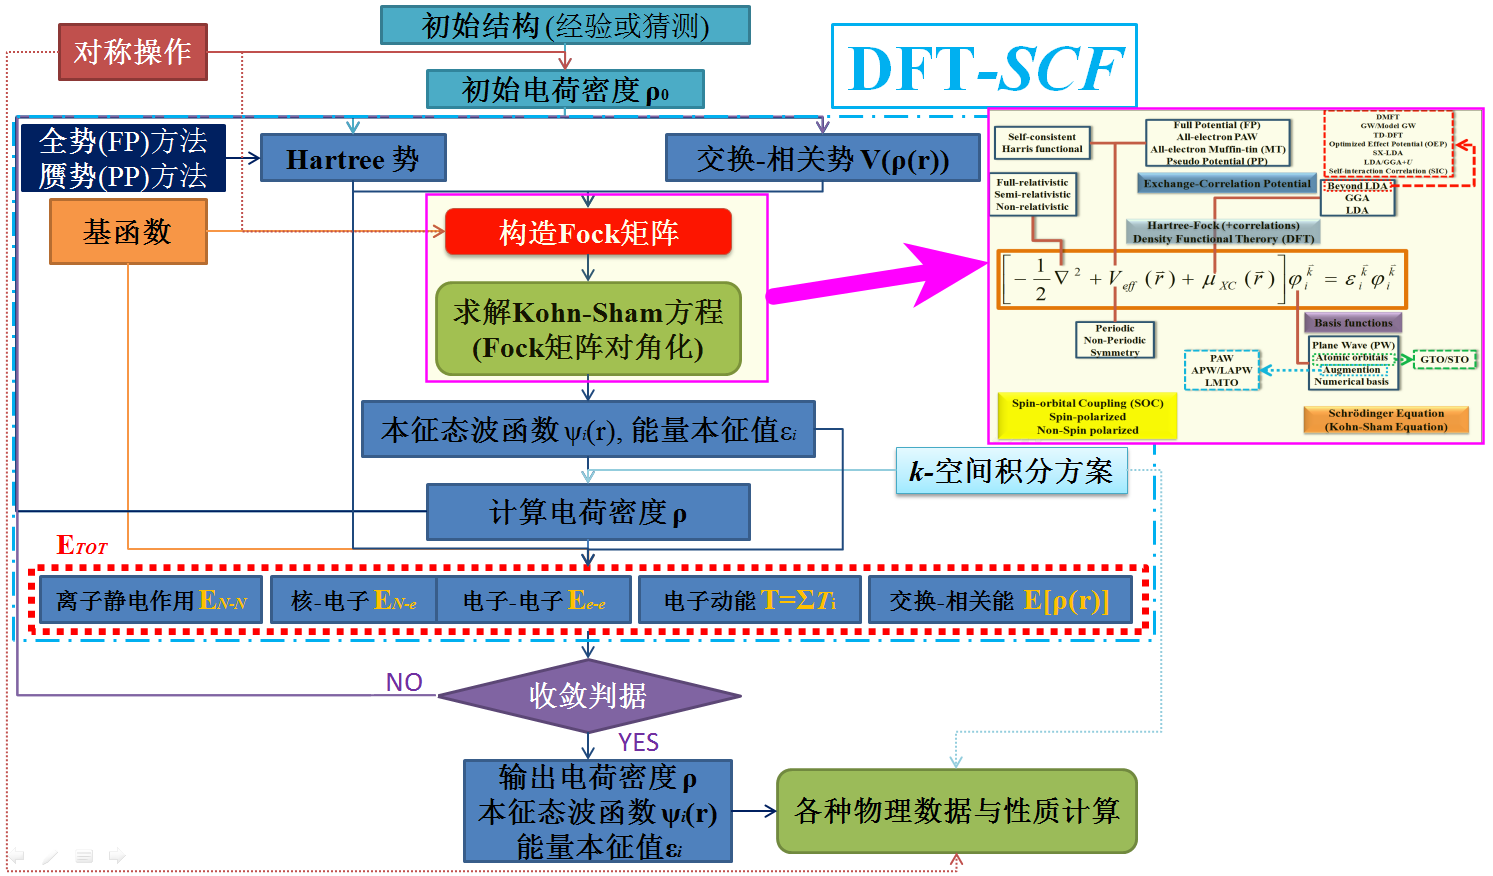
\includegraphics[height=2.80in,width=4.95in,viewport=5 3 1490 870,clip]{Figures/DFT-SCF_2.png}
%\caption{\tiny \textrm{Pseudopotential for metallic sodium, based on the empty core model and screened by the Thomas-Fermi dielectric function.}}%(与文献\cite{EPJB33-47_2003}图1对比)
\label{DFT-SCF-2}
\end{figure}
}

\frame                               %
{
	\frametitle{\textrm{Kohn-Sham}方程}
\begin{figure}[h!]
\centering
\vspace*{-0.21in}
\hspace*{-0.1in}
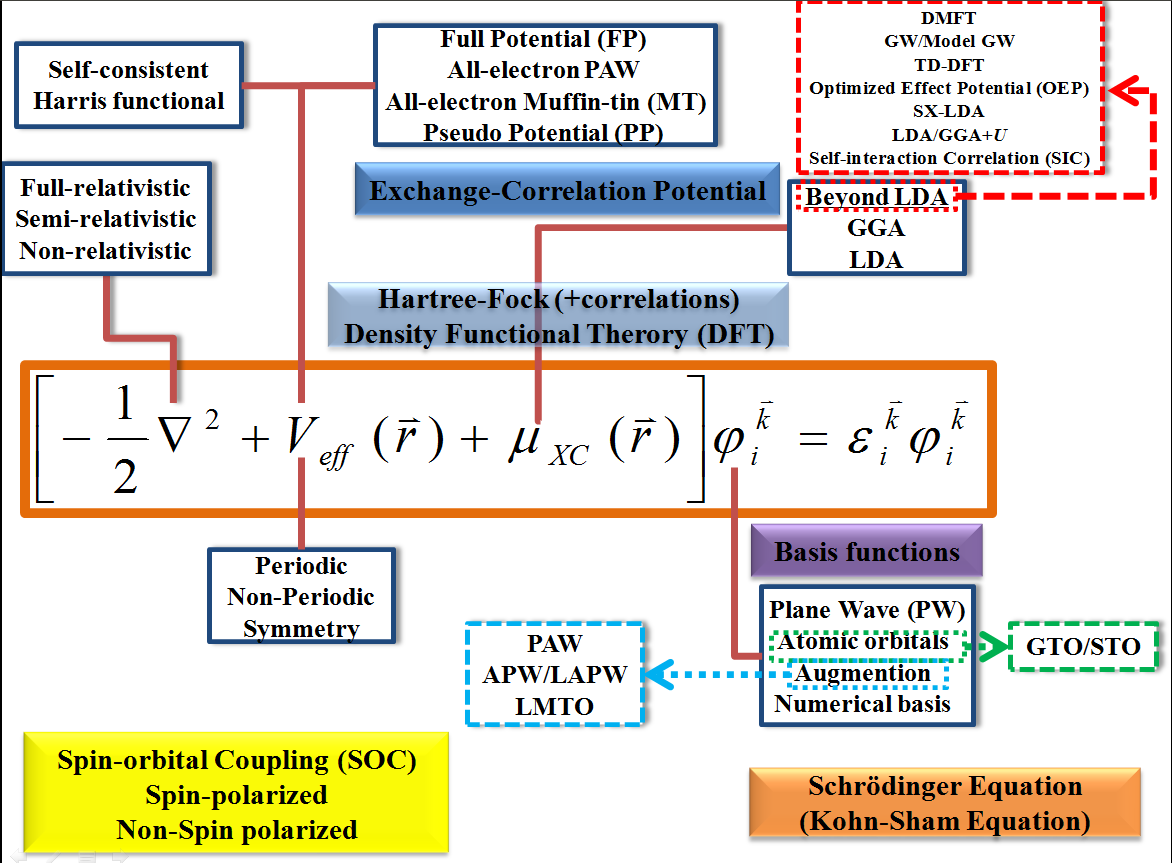
\includegraphics[height=2.7in,width=4.0in,viewport=2 5 1162 880,clip]{Figures/DFT.png}
\caption{\tiny \textrm{The Analysis of Kohn-Sham equation.}}%(与文献\cite{EPJB33-47_2003}图1对比)
\label{DFT}
\end{figure}
}

\section{赝势理论}       %Bookmark
%\section{Induction on DFT and solid-state physics}       %Bookmark
\frame
{
	\frametitle{球形势对平面波的散射与相移}
\begin{figure}[h!]
\centering
\vspace*{-0.26in}
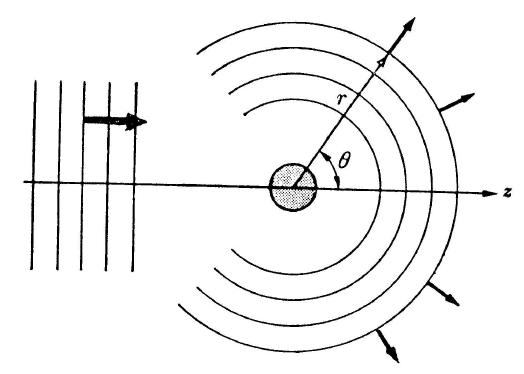
\includegraphics[height=0.90in,width=1.24in,viewport=0 0 400 300,clip]{Figures/Pseudo-scatter.jpg}
\caption{\fontsize{5.5pt}{4.2pt}\selectfont{\textrm{Schematic illustration of scattering of a plane wave by a spherical potential.}}}%(与文献\cite{EPJB33-47_2003}图1对比)
\label{Pseudo-scatter}
\end{figure}
\vspace*{-0.1in}
\fontsize{7.5pt}{6.2pt}\selectfont{
入射平面波
$$\mathrm{e}^{\mathrm{i}\vec q\cdot\vec r}=4\pi\sum_{lm}\mathrm{i}^lj_l(\vec q\cdot\vec r)Y_{lm}^{\ast}(\hat{\vec q})Y_{lm}(\hat{\vec r})=\sum_{l}(2l+1)\mathrm{i}^lj_l(qr)P_{l}(\cos\theta)$$
%$$\mathrm{e}^{\mathrm{i}\vec q\cdot\vec r}=\mathrm{e}^{\mathrm{i}qr\cos(\theta)}=\sum_{l}(2l+1)\mathrm{i}^lj_l(qr)P_{l}[\cos(\theta)]$$
经散射后出射,波函数变为
$$\Psi_l^{>}(\varepsilon,r)=C_l\bigg[j_l(\kappa r)-\tan\eta_l(\varepsilon)n_l(\kappa r)\bigg]\quad\text{其中}\kappa^2=\varepsilon$$
根据散射理论,能量为$\varepsilon$的电子经单个势阱散射偏转$\theta$后,波函数的振幅可以表示为
	\begin{displaymath}
		t(\theta)=\dfrac{4\pi}{\kappa}\sum_l(2l+1)[\mathrm{exp}(2\mathrm{i}\eta_l(\varepsilon))-1]P_l(\cos\theta)
	\end{displaymath}
%$$t(\theta)=\dfrac{4\pi}{\sqrt\varepsilon}\sum_l(2l+1)\bigg[\mathrm{e}^{2\mathrm{i}\eta_l(\varepsilon)}-1\bigg]P_l(\cos\theta)$$
%$$\eta_l(\varepsilon)=p_l\pi+\delta_l(\varepsilon)$$
}
}

\frame
{
	\frametitle{散射相移与赝势}
\begin{figure}[h!]
\centering
\vspace*{-0.25in}
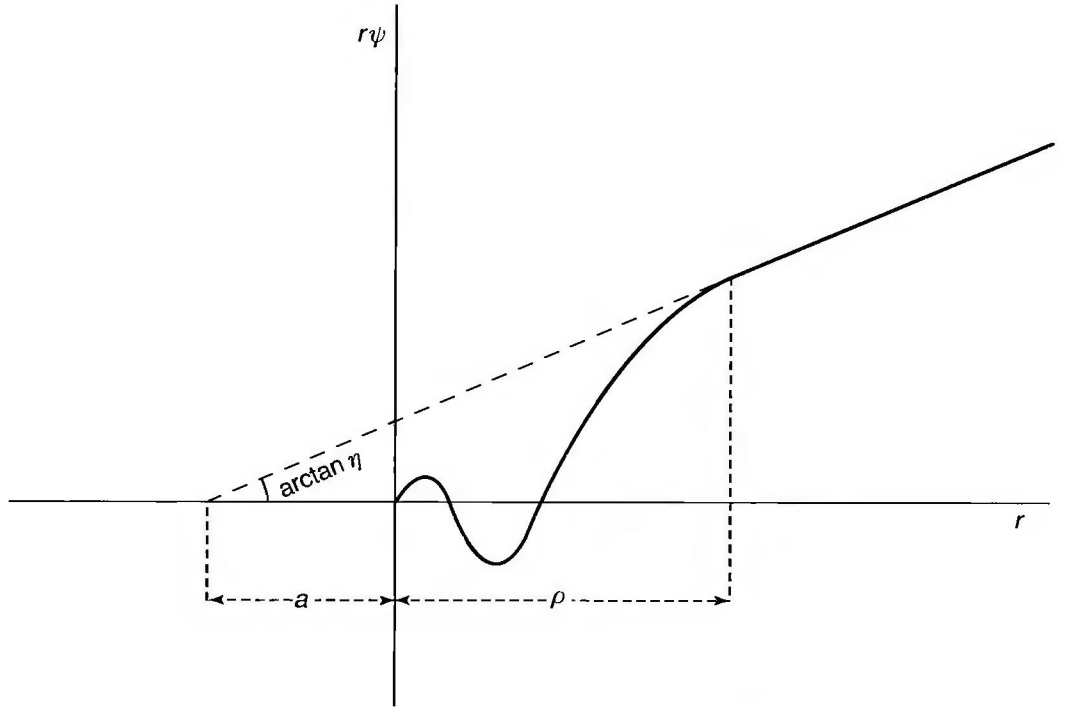
\includegraphics[height=1.20in,width=1.77in,viewport=0 0 1150 750,clip]{Figures/Pseudo-scatter-2.png}
\caption{\fontsize{4.5pt}{3.2pt}\selectfont{\textrm{Radial wave-function $\phi=r\psi$ for low-energy scattering as illustrated in a figure from the 1934 and 1935 papers of Fermi and coworkers for low-energy electron scattering from atoms and neutron scattering from nuclei. The node in the wave-function near the origin show that the potential is attractive and strong enough to have bound states. The cross-section for scattering from the localized potential is determined by the phase shift and is the same for weaker pseudo-potential with the same phase shift modulo $2\pi$.}}}%(与文献\cite{EPJB33-47_2003}图1对比)
\label{Pseudo-scatter-2}
\end{figure}
\fontsize{7.5pt}{6.2pt}\selectfont{
对于球形势散射,相移可由径向波函数计算
$$\tan\eta_l(\varepsilon)=\dfrac{R\frac{\mathrm{d}}{\mathrm{d}r}j_l(\kappa r)|_R-D_l(\varepsilon)j_l(\kappa R)}{R\frac{\mathrm{d}}{\mathrm{d}r}n_l(\kappa r)|_R-D_l(\varepsilon)n_l(\kappa R)}$$
$$\mbox{其中~}D_l(\varepsilon,r)\equiv r\psi_l^{\prime}(r)/\psi_l(r)=r\dfrac{\mathrm{d}}{\mathrm{d}r}\ln\psi_l(r)$$
同时相移与波函数节点的关系为:$$\eta_l(\varepsilon)=p_l\pi+\delta(\varepsilon)$$}
}

\subsection{平面波与赝势}       %Bookmark
\frame
{
%\frametitle{The methods on band structure calculation}
	\frametitle{由\textrm{OPW~}到赝势}
%\vskip 10pt
%\textrm{The mainly difference of all these methods below: the basis sets and the construction of the potential}
\begin{itemize}
%\setlength{\itemsep}{5pt}
	\item 完全平面波基组\\{\fontsize{7.5pt}{5.5pt}\selectfont{少数平面波就可以很好地描述波函数在原子间的行为,近核波函数则需要大量平面波展开}}%。因此完全平面波基组虽然方便,但求体系本征态对角化的矩阵非常巨大,计算变得异常耗时。
	\item 正交平面波(\textrm{Orthogonalized plane wave, OPW})方法\\{\fontsize{7.5pt}{5.5pt}\selectfont{价电子用与芯层波函数正交的平面波展开
		\begin{displaymath}
			\phi_{\textrm{OPW}}^{\vec k+\vec G}(\vec r)=\phi_{\textrm{PW}}^{\vec k+\vec G}(\vec r)-\sum_c\langle\varphi_c|\phi_{\textrm{PW}}^{\vec k+\vec G}\rangle\varphi_c(\vec r)
		\end{displaymath}}}
	{\fontsize{7.5pt}{5.5pt}\selectfont{构造赝波函数
		\begin{displaymath}
			\tilde{\phi}_v(\vec r)=\phi_v(\vec r)+\sum_c\langle\varphi_c|\tilde{\phi}_v\rangle\varphi_c(\vec r)
		\end{displaymath}
	代入\textrm{Schr\"odinger}方程
		$$\hat H|\tilde{\phi}_v\rangle-\sum_c\langle\varphi_c|\tilde{\phi}_v\rangle\hat H|\varphi_c\rangle=\varepsilon_v|\tilde{\phi}_v\rangle-\varepsilon_v\sum_c\langle\varphi_c|\tilde{\phi}_v\rangle|\varphi_c\rangle$$
		可有$$\hat H|\tilde{\phi}_v\rangle+\textcolor{blue}{V^R}|\tilde{\phi}_v\rangle=\textcolor{blue}{\varepsilon_v}|\tilde{\phi}_v\rangle$$
		这里排斥势是$$V^R(\vec r,\vec r^{\prime})=\sum_c(\varepsilon_v-\varepsilon_c)|\varphi_c(\vec r^{\prime})\rangle\langle\varphi_c(\vec r)|$$}}
\end{itemize}
}

\frame
{
	\frametitle{由\textrm{OPW~}到赝势}
	\textrm{Phillips-Kleinman}指出,赝势($V^{e\!f\!f}$)-赝波函数(可用$\phi_{PW}^{\vec k+\vec G}$展开)满足\textrm{Schr\"odinger}方程%\upcite{PR116-287_1959}
	$$\bigg(-\dfrac12\nabla^2+\textcolor{red}{V^{e\!f\!f}}\bigg)|\tilde{\phi}_v\rangle=\textcolor{blue}{\varepsilon_v}|\tilde{\phi}_v\rangle$$
	其中$\textcolor{red}{V^{e\!f\!f}}=V(\vec r)+\textcolor{blue}{V^R}$
	\begin{itemize}
		\item 赝势-赝波函数的本征值$\varepsilon_v$与真实体系的价电子能量本征值等价
		\item 赝势$\textcolor{red}{V^{e\!f\!f}}$比$V(\vec r)$平滑得多,并且$\textcolor{blue}{V^R}$是非局域的排斥势
			\begin{displaymath}
				\begin{aligned}
					\textcolor{blue}{V^R}f(\vec r)=&\sum_c(\varepsilon_v-\varepsilon_c)\varphi_c(\vec r)\int\varphi_c^{\ast}(\vec r^{\prime})f(\vec r^{\prime})\mathrm{d}\vec r^{\prime} \\
					=&\int V^R(\vec r,\vec r^{\prime})f(\vec r^{\prime})\mathrm{d}\vec r^{\prime}
				\end{aligned}
			\end{displaymath}
%			这里$$V^R(\vec r,\vec r^{\prime})=\sum_c(\varepsilon_v-\varepsilon_c)|\varphi_c(\vec r^{\prime})\rangle\langle\varphi_c(\vec r)|$$
	\end{itemize}
}

\frame
{
\frametitle{赝势的评估}
赝势(\textrm{Pseudo Potential, PP})方法是在正交平面波的基础上发展起来的,构造出平缓的势函数代替核的强吸引作用和芯层电子的排斥作用,用平缓的函数取代波函数近核时的震荡。
\begin{itemize}
\setlength{\itemsep}{5pt}
	\item 赝势-平面波方法,只需要少量平面波可展开赝波函数,大大提升了计算效率;但是赝波函数不能很好地反映与电子近核行为有关的性质。
	\item 赝势的构造并不唯一,考核构造赝势的两大指标:~\\“柔软程度”\textrm{(Soft)}与“可移植性”\textrm{(transferability)}
\end{itemize}
\begin{figure}[h!]
\centering
\vspace*{-0.10in}
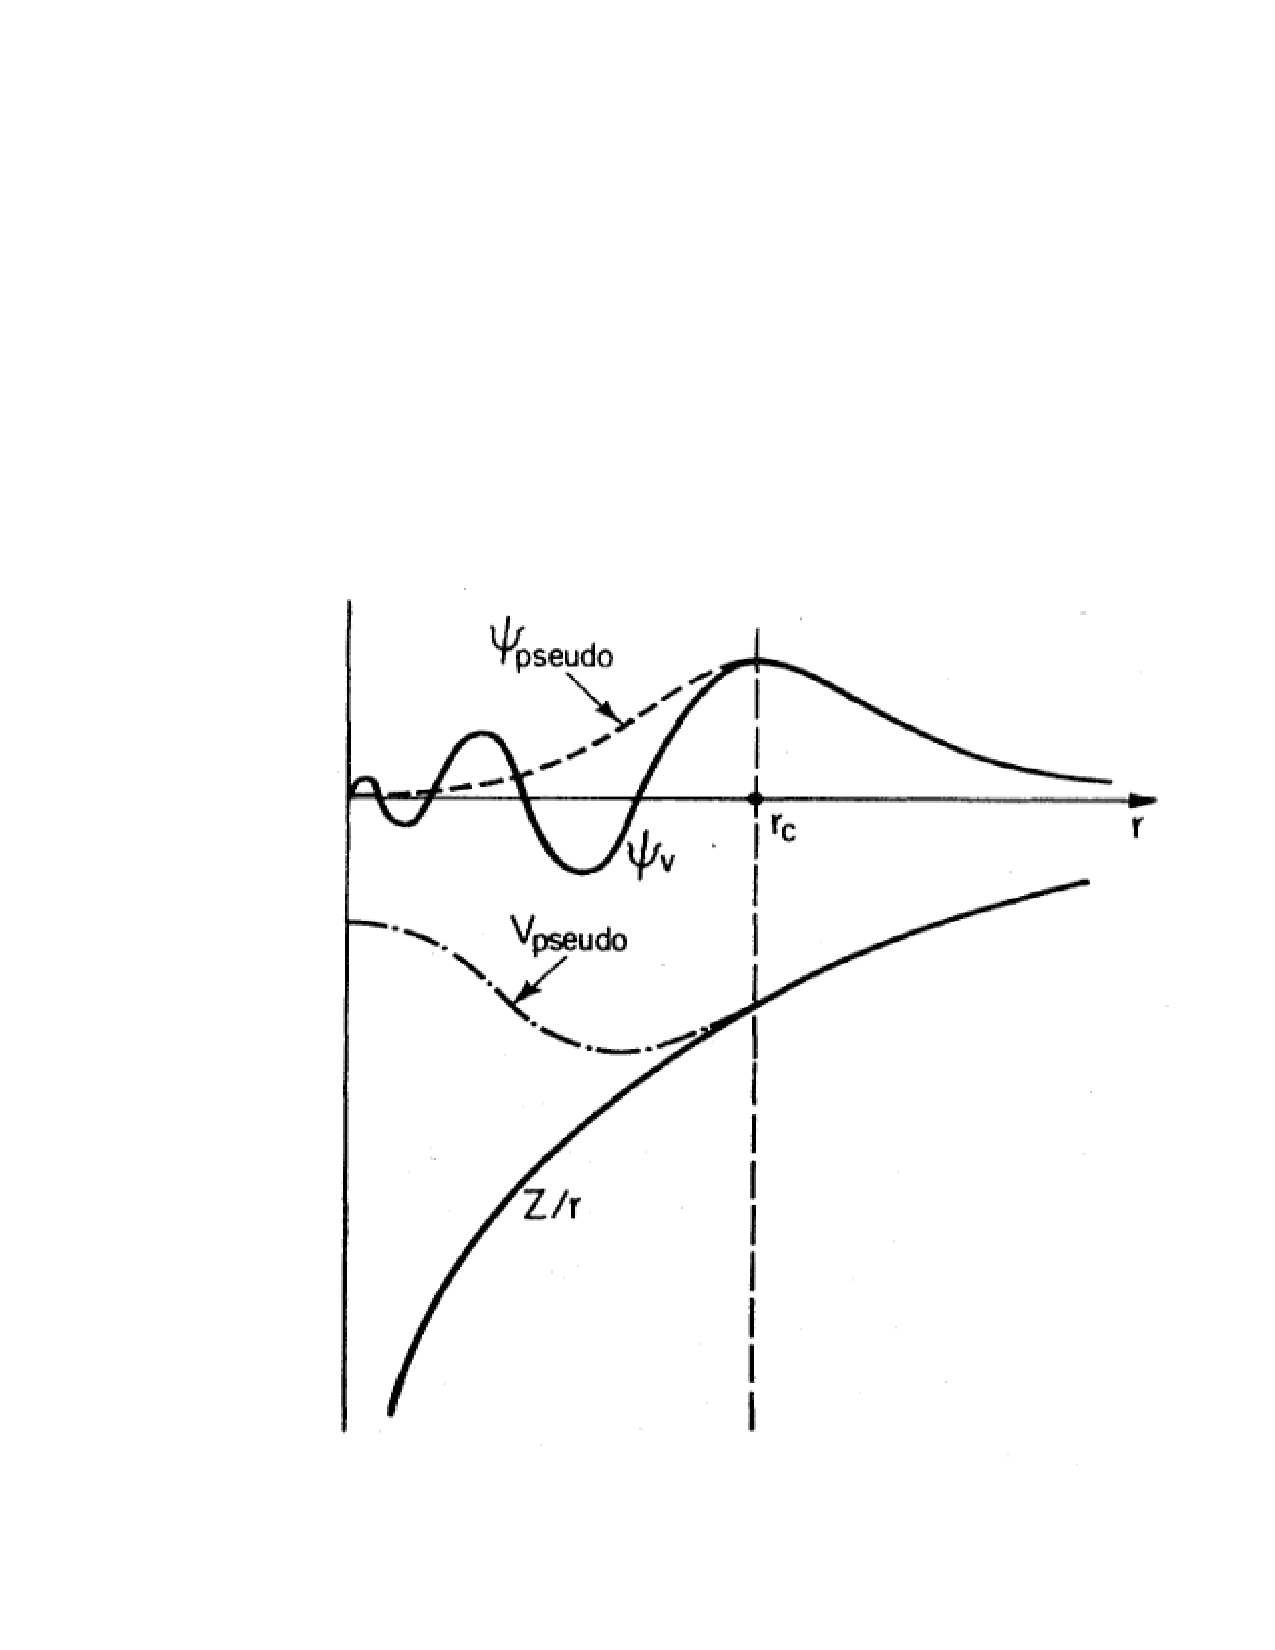
\includegraphics[height=1.35in,width=1.40in,viewport=154 100 562 508,clip]{Figures/Pseudo.pdf}
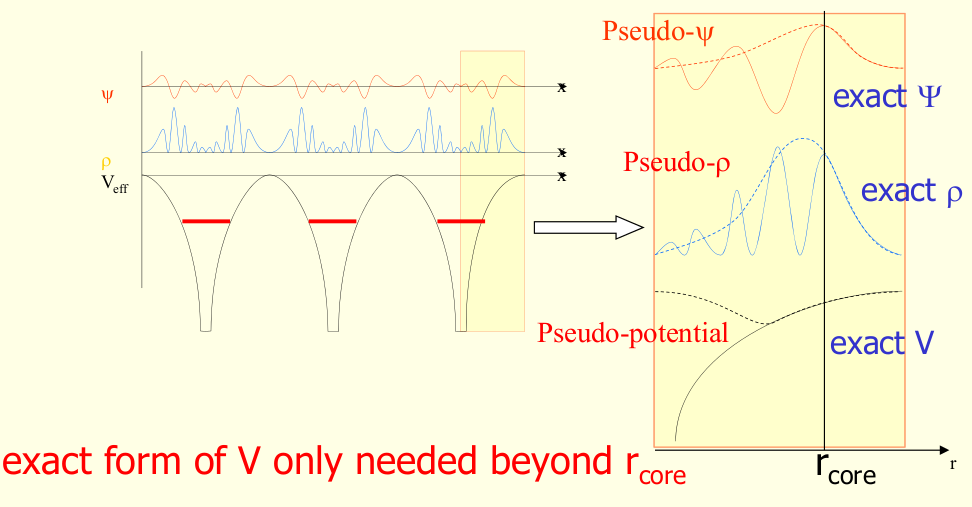
\includegraphics[height=1.35in,width=2.55in,viewport=1 1 980 500,clip]{Figures/Pseudo-2.png}
\caption{\tiny \textrm{The Pseudo wave function and Pseudo potential.}}%(与文献\cite{EPJB33-47_2003}图1对比)
\label{Pseudo_Potential-Wave}
\end{figure}
}

\frame
{
	\frametitle{传统赝势的构造}
	直接由实验数据来确定(模型)赝势,常用的实验数据包括离子对电子的散射角度、离子的光谱实验数据等
		\begin{itemize}
			\item 构造离子赝势:~可移植性好
			\item 构造总赝势(包括全部价电子相互作用):~常用于能带描述
		\end{itemize}
%	\begin{itemize}
%		\item 在指定能量范围内,离子对电子散射的散射角
%		\item 离子的光谱实验数据
%	\end{itemize}
\begin{figure}[h!]
\centering
\vspace*{-0.10in}
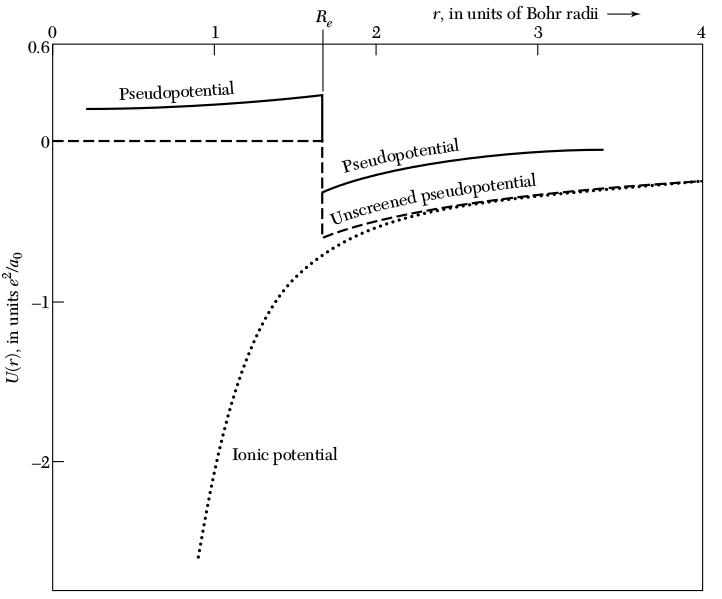
\includegraphics[height=1.60in,width=2.57in,viewport=0 0 980 600,clip]{Figures/Pseudo-model-empty_core.png}
\caption{\tiny \textrm{Pseudopotential for metallic sodium, based on the empty core model and screened by the Thomas-Fermi dielectric function.}}%(与文献\cite{EPJB33-47_2003}图1对比)
\label{Pseudo_model-empty_core}
\end{figure}
}

\frame
{
	\frametitle{传统赝势的构造}
\begin{figure}[h!]
\centering
\vspace*{-0.10in}
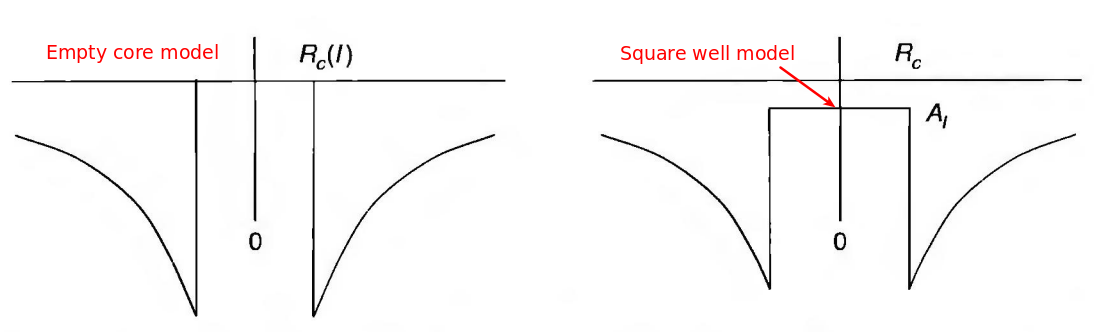
\includegraphics[height=1.30in,width=4.17in,viewport=0 0 1150 350,clip]{Figures/Pseudo-model.png}
\caption{\tiny \textrm{Left:``Empty core'' model potential of Ashcroft in which the potential is zero inside radius $R_c(l)$ which is different for each $l$. Right: Square well model potential with value $A_l$ inside a cut-off radius $R_c$, proposed by Abarenkov and Heine and fit to atomic data by Animalu and Heine. The fact that the potential are weak, zero, or even positive inside cut-off radius $R_c$ is an illustration of the ``cancellation theorem''.}}%(与文献\cite{EPJB33-47_2003}图1对比)
\label{Pseudo-model}
\end{figure}
}

\subsection{模守恒赝势}
\frame
{
	\frametitle{第一原理赝势}
		由第一原理求解出全电子波函数(径向部分)$P_{n,l}(r)$
			\begin{displaymath}
				\bigg[-\dfrac12\dfrac{\mathrm{d}^2}{\mathrm{d}r^2}+\dfrac{l(l+1)}{2r^2}+V(\rho,r)\bigg]P_{n,l}(r)=\varepsilon_{n,l}P_{n,l}(r)
			\end{displaymath}
			这里$V(\rho,r)$是自洽单电子势
			$$V(\rho,r)=-\frac{Z}r+V_{\mathrm H}(\rho,r)+V_{XC}^{\mathrm{LDA}}(\rho(r))$$
			$V_{\mathrm H}(\rho,r)$是\textrm{Hartree}势,$V_{XC}^{\mathrm{LDA}}(\rho(r))$是交换-相关势

			由此构造赝波函数$P_l^{\mathrm{PP}}(r)$,满足
			$$P_l^{\mathrm{PP}}(r)=P_l^{\mathrm{AE}}(r),\quad r>r_{l}^c$$
			进而构造赝势$V_{\mathrm{src},l}^{\mathrm{PP}}(r)$
			$$V_{\mathrm{src},l}^{\mathrm{PP}}(r)=\varepsilon_l-\dfrac{l(l+2)}{2r^2}+\dfrac{1}{2P_l^{\mathrm{PP}}(r)}\dfrac{\mathrm{d}^2}{\mathrm{d}r^2}P_l^{\mathrm{PP}}(r),\quad r<r_{l}^c$$
}

\frame
{
	\frametitle{模守恒\textrm{(Norm-conserving)}条件}
%	构造赝势确定参数的边界(构造条件)
	\begin{enumerate}
		\item 价电子赝波函数的能量本征值与对应全电子波函数能量本征值相等:~$\varepsilon_l^{\mathrm{PP}}=\varepsilon_l^{\mathrm{AE}}$
		\item 价电子赝波函数与真实电子波函数的径向部分在截断半径$r_{c,l}$外相同:~$\psi_l^{\mathrm{PP}}(r)=\psi_l^{\mathrm{AE}}(r),\quad r>r_{l}^c$
		\item 价电子赝波函数与真实电子波函数的对数导数在截断半径$r_{c,l}$处相等:~$D_l^{\mathrm{PP}}(r)=D_l^{\mathrm{AE}}(r),\quad r\geqslant r_{l}^c$\\
		这里$D_l(\varepsilon,r)=r\frac{\psi_l^{\prime}(\varepsilon,r)}{\psi_l(\varepsilon,r)}=r\dfrac{\mathrm{d}}{\mathrm{d}r}\ln\psi_l(\varepsilon,r)$
		\item 价电子赝波函数与真实电子波函数在截断半径$r_{l}^c$内的积分电荷相等(\textcolor{red}{模守恒条件})
			$$Q_l=\int_0^{r_{l}^c}\mathrm{d}rr^2|\psi_l^{\mathrm{PP}}(r)|^2=\int_0^{r_{l}^c}\mathrm{d}rr^2|\psi_l^{\mathrm{AE}}(r)|^2$$
		\item 价电子赝波函数与真实电子波函数的对数导数一阶能量导数$\mathrm{d}D_l(\varepsilon,r)/\mathrm{d}\varepsilon$在截断半径$r_{l}^c$处及以外相等
	\end{enumerate}
}

\frame
{
	\frametitle{模守恒\textrm{(Norm-conserving)}条件}
\begin{figure}[h!]
\centering
\vspace*{-0.10in}
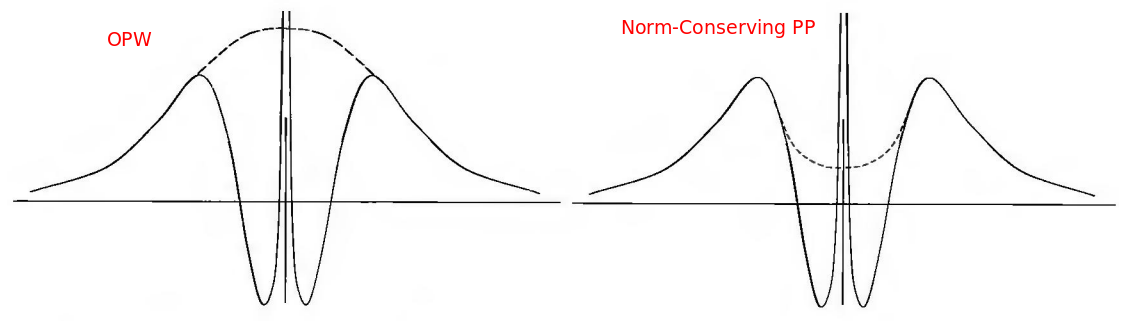
\includegraphics[height=1.30in,width=4.17in,viewport=0 0 1150 350,clip]{Figures/Pseudo-OPW_NCPP.png}
\caption{\tiny \textrm{Schematic example of a valence function that has the character of a $3s$ orbital near the nucleus and two examples of smooth functions (dashed lines) that equal the full wave-function outside the core region. Left: the smooth part of the valence function defined by OPW-like equation; Right: a smooth pseudo-function that satisfies the norm-conservation condition.}}%(与文献\cite{EPJB33-47_2003}图1对比)
\label{Pseudo-OPW_NCPP}
\end{figure}
}

\frame
{
	\frametitle{赝势去屏蔽}
	第一原理赝势建立了赝波函数与对应赝势的一一对应关系,但该赝势包含了电子屏蔽(原子、离子环境)信息,去屏蔽后的赝势对环境依赖更低,“可移植性”更好
	$$V_{\mathrm{ion},l}^{\mathrm{PP}}(r)=V_{\mathrm{src},l}^{\mathrm{PP}}(r)-V_{\mathrm{H},l}^{\mathrm{PP}}(r)-V_{XC,l}^{\mathrm{PP}}(r)$$
	去屏蔽过程中,特别需要注意$V_{XC,l}^{\mathrm{PP}}(r)$的处理
	$$V_{XC,l}^{\mathrm{PP}}(r)=V_{XC}^{\mathrm{PP}}([n_l^{\mathrm{PP}}],r)+\big[V_{XC}^{\mathrm{PP}}([n_l^{\mathrm{PP}}+n^{core}],r)-V_{XC}^{\mathrm{PP}}([n_l^{\mathrm{PP}}],r)\big]$$
}

\frame
{
	\frametitle{非局域赝势}
	当前第一原理赝势径向部分是局域的,但与$l$有关,因此是半局域的(\textrm{semi-local})
	\begin{displaymath}
		\hat{V}^{\mathrm{SL}}=\sum_{lm}|Y_{lm}\rangle V_l(r)\langle Y_{lm}|
	\end{displaymath}
	将赝势的径向部分分解为局域部分($l$无关)和非局域部分($l$相关)
	\begin{displaymath}
		V_{\mathrm{ion},l}^{\mathrm{PP}}(r)=V_{\mathrm{local}}^{\mathrm{PP}}(r)+\delta V_l^{\mathrm{PP}}(r)
	\end{displaymath}
	第一原理赝势可以表示为
	\begin{displaymath}
		\hat{V}^{\mathrm{SL}}=V_{\mathrm{local}}^{\mathrm{PP}}(r)+\sum_{lm}|Y_{lm}\rangle\delta V_l(r)\langle Y_{lm}|
	\end{displaymath}
	赝势的非局域部分可以表示为
	\begin{displaymath}
		\delta V(\vec r,\vec r^{\prime})=\sum_{lm}|Y_{lm}\rangle\delta V_l(r)\langle Y_{lm}|
	\end{displaymath}
}

\frame
{
	\frametitle{模守恒赝势构造流程}
\begin{figure}[h!]
\centering
%\vspace*{-0.10in}
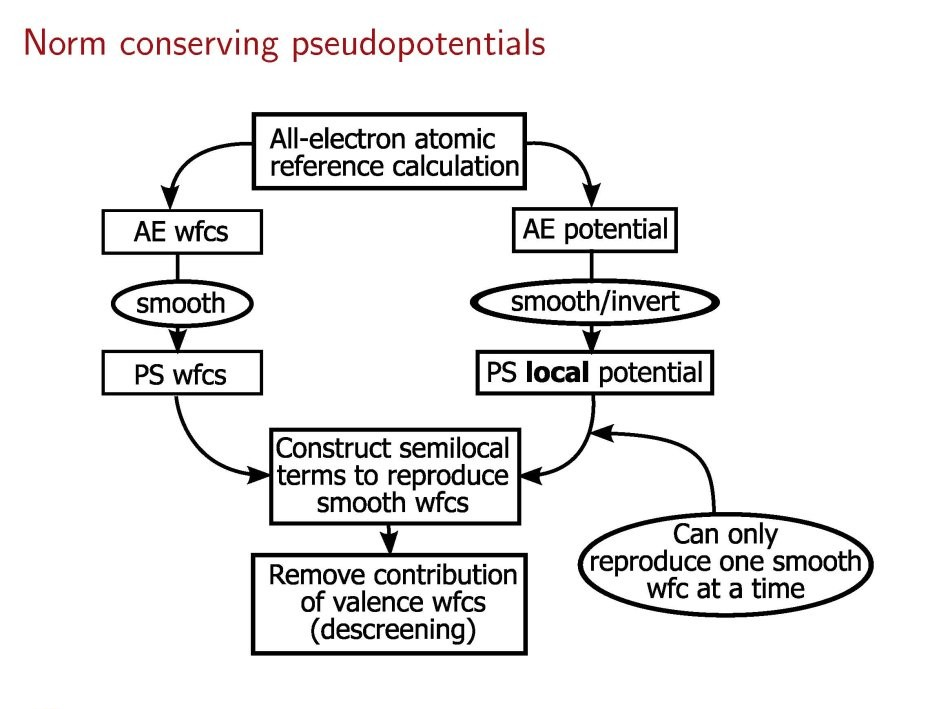
\includegraphics[height=2.70in,width=3.77in,viewport=70 40 900 610,clip]{Figures/Pseudo-NC.jpg}
%\caption{\tiny \textrm{Pseudopotential for metallic sodium, based on the empty core model and screened by the Thomas-Fermi dielectric function.}}%(与文献\cite{EPJB33-47_2003}图1对比)
\label{Pseudo-NC}
\end{figure}
}

\subsection{可分离赝势与\rm{Ghost~band}}
\frame
{
	\frametitle{非局域赝势的变量分离}
	\textrm{Kleinman-Bylander}提出了非局域赝势的变量分离的近似方案\footnote{即$\delta V(\vec r,\vec r^{\prime})$可以写成$\delta V(\vec r,\vec r^{\prime})=\sum_{i}f_i(\vec r)g_i(\vec r^{\prime})$的形式}:~\\
%	引入分离算符$\delta V^{\mathrm{NL}}$满足
	{\fontsize{7.2pt}{5.2pt}\selectfont{如果选择适当的局域函数$V_{\mathrm{local}}^{\mathrm{PP}}(r)$,赝势将可分解为局域部分与非局域部分之和:
	$$\hat V_{\mathrm{NL}}^{\mathrm{PP}}(r)=V_{\mathrm{local}}^{\mathrm{PP}}(r)+\sum_{lm}\dfrac{|\psi_{lm}^{\mathrm{PP}}\delta V_l\rangle\langle\delta V_l\psi_{lm}^{\mathrm{PP}}|}{\langle\psi_{lm}^{\mathrm{PP}}|\delta V_l|\psi_{lm}^{\mathrm{PP}}\rangle}$$ 
	\textcolor{magenta}{$\langle\delta V_l(r)\psi_{lm}^{\mathrm{PP}}|$是投影子},这种分解称为\textrm{factored pseudo-potential},方便数值计算
\vskip 10pt
	更一般地,如果允许赝势局域部分$V_{\mathrm{local}}^{\mathrm{PP}}(r)$为任意函数,则可定义辅助函数
	$$\chi_{lm}^{\mathrm{PP}}(\vec r)=\bigg\{\varepsilon_l-\bigg[-\dfrac12\nabla^2+V_{\mathrm{local}}^{\mathrm{PP}}(\vec r)\bigg]\bigg\}\psi_{lm}^{\mathrm{PP}}(\vec r)$$
	于是赝势的非局域部分可表示为
	$$\delta V_{\mathrm{NL}}=\sum_{lm}\dfrac{|\chi_{lm}^{\mathrm{PP}}\rangle\langle\chi_{lm}^{\mathrm{PP}}|}{\langle\chi_{lm}^{\mathrm{PP}}|\psi_{lm}^{\mathrm{PP}}\rangle}$$
但是$V_{\mathrm{local}}^{\mathrm{PP}}(r)$选择的随意性,将增加计算结果出现\textrm{Ghost~band}的风险
}}
}

\frame
{
	\frametitle{\textrm{Ghost~band}的表现}
	\fontsize{9.2pt}{4.2pt}\selectfont{只有价电子的赝波函数与芯电子波函数完全正交,能带计算中才能确保芯层与价层电子的完全分离。但实际计算时,该正交条件很难严格保证,因此一旦赝波函数严重偏离正交条件,计算的能带中会在本不存在能带的区域出现电子结构分布(称为\textrm{Ghost~band}),这部分电子结构源自构造赝波函数的能量参数$\varepsilon_l$与芯层电子能量差别太大,无法保持与芯层电荷严格正交引起的}
\begin{figure}[h!]
\centering
\vspace*{-0.10in}
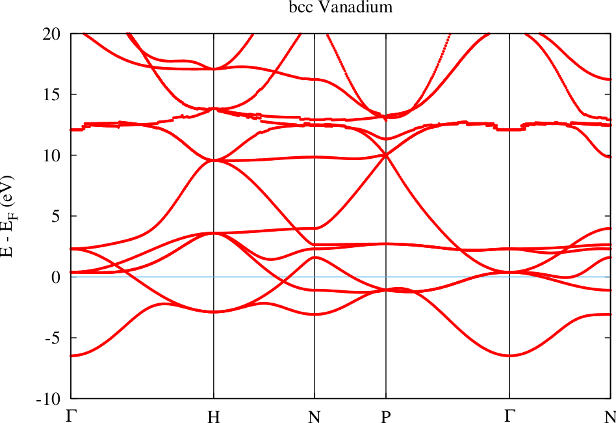
\includegraphics[height=1.50in,width=1.98in,viewport=0 0 450 320,clip]{Figures/Ghostband-Vanadium-1.png}
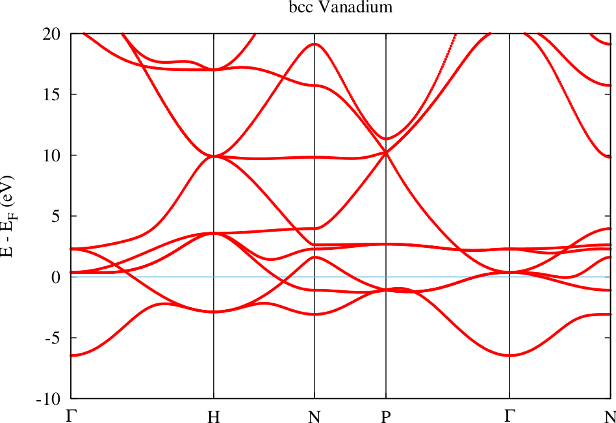
\includegraphics[height=1.50in,width=1.98in,viewport=0 0 450 320,clip]{Figures/Ghostband-Vanadium-4.png}
\caption{\fontsize{7.2pt}{4.2pt}\selectfont{\textrm{The band structure of bcc Vanadium. %In the calculation, all electrons up to the 3p states were treated as core electrons, all other electrons as valence electrons. 
\\Left:~Between 10 and 15 eV above the Fermi energy a strange band with nearly no dispersion can be observed. The vanishing dispersion of the band is a typical property of ghost bands.}}}%(与文献\cite{EPJB33-47_2003}图1对比)
\label{Ghost-band}
\end{figure}
}

\frame
{
	\frametitle{\textrm{Ghost~band}的根源}
	可分离赝势方法中
	\begin{displaymath}
		\hat{\mathbf{H}}=-\dfrac12\nabla^2+V_{\mathrm{local}}(r)+\delta\hat{V}_{\mathrm{NL}}
	\end{displaymath}
	赝波函数$\psi_{lm}^{\mathrm{PP}}(r)$是方程
	\begin{displaymath}
		\hat{\mathbf{H}}\psi_{lm}^{\mathrm{PP}}(r)=\varepsilon_l\psi_{lm}^{\mathrm{PP}}(r)
	\end{displaymath}
	的解。
\vskip 15pt
	因为$V_{\mathrm{local}}(r)$可随意选择,因此赝波函数$\psi_{lm}^{\mathrm{PP}}(r)$和能量$\varepsilon_l$不再要求与束缚态波函数相对应,将导致\textrm{Ghost~band}的出现
}

\frame
{
	\frametitle{\textrm{Ghost~band}根源的数学说明$^{\ast}$}
	{\fontsize{7.2pt}{5.2pt}\selectfont{对于半局域势,求解能量$\varepsilon$对应的径向波函数$u_l(r,\varepsilon)$的方程\textcolor{blue}{是一个常微分方程}
		\begin{displaymath}
			-\dfrac12\dfrac{\mathrm{d}^2u_l}{\mathrm{d}r^2}+\overline{V}_l^{\mathrm{loc}}(r)u_l(r,\varepsilon)+\Delta V_l^{\mathrm{SL}}(r)u_l(r,\varepsilon)-\varepsilon u_l(r,\varepsilon)=0
		\end{displaymath}
		而对于可分离赝势(如\textrm{KB}势),方程则为\textcolor{blue}{积分-微分方程}
		\begin{displaymath}
			-\dfrac12\dfrac{\mathrm{d}^2u_l}{\mathrm{d}r^2}+\overline{V}_l^{\mathrm{loc}}(r)u_l(r,\varepsilon)+\int\Delta V_l(r,r^{\prime})u_l(r^{\prime},\varepsilon)\mathrm{d}r^{\prime}-\varepsilon u_l(r,\varepsilon)=0
		\end{displaymath}
		将可分离赝势代入可有
		\begin{displaymath}
			-\dfrac12\dfrac{\mathrm{d}^2u_l}{\mathrm{d}r^2}+\overline{V}_l^{\mathrm{loc}}(r)u_l(r,\varepsilon)+f_l(r)\int g_l(r^{\prime})u_l(r^{\prime},\varepsilon)\mathrm{d}r^{\prime}-\varepsilon u_l(r,\varepsilon)=0
		\end{displaymath}
		\begin{itemize}
			\item \textcolor{blue}{常微分方程解的结构服从\textrm{Wronskian}定理的推论:~本征态能量$\varepsilon_0,\varepsilon_1,\cdots,\varepsilon_n$按升序排列时,对应的本征态波函数(径向)的节点数依次递增}
			\item \textcolor{red}{积分-微分方程解的结构不要求满足该结论:~波函数的节点数与能量本征态不再有对应的升序关系}
		\end{itemize}
		由于积分项的存在,传统的常微分方程求解算法(如\textrm{Runger-Kutta}法等)无法直接用于该积分-微分方程,必须另图别策
	}}
}

\frame
{
	\frametitle{\textrm{Ghost~band}根源的数学说明$^{\ast}$}
		{\fontsize{7.2pt}{5.2pt}\selectfont{
		基本思想:~类似积分方程求解的\textrm{Fredholm}方法
		\begin{itemize}
			\item 先将微分方程中的\textcolor{magenta}{积分项近似为常数因子},\textcolor{blue}{求解非齐次常微分方程}
			\item 对含有波函数的积分,应用闭路积分公式\textrm{(closure formula)}计算
		\end{itemize}}}
		{\fontsize{5.2pt}{5.2pt}\selectfont{具体求解流程
		\begin{enumerate}
			\item 采用通用方法分别求解\\\textcolor{blue}{齐次微分方程}
				\begin{displaymath}
					-\dfrac12\dfrac{\mathrm{d}^2W_l}{\mathrm{d}r^2}+\overline{V}_l^{\mathrm{loc}}(r)W_l(r,\varepsilon)-\varepsilon W_l(r,\varepsilon)=0
				\end{displaymath}
				的通解和\\\textcolor{magenta}{不含积分项的}\textcolor{blue}{非齐次微分方程}
				\begin{displaymath}
					-\dfrac12\dfrac{\mathrm{d}^2X_l}{\mathrm{d}r^2}+\overline{V}_l^{\mathrm{loc}}(r)X_l(r,\varepsilon)-\varepsilon X_l(r,\varepsilon)=f_l(r)
				\end{displaymath}
				的一个特解
			\item 构造积分
				\begin{displaymath}
					\begin{aligned}
					\tilde {W}(\varepsilon)=&\int g_l(r)W(r,\varepsilon)\mathrm{d}r\\
					\tilde {X}(\varepsilon)=&1+\int g_l(r)X(r,\varepsilon)\mathrm{d}r
					\end{aligned}
				\end{displaymath}
			\item 由此得到积分-微分方程的解
				\begin{displaymath}
					u(r,\varepsilon)=K[W(r,\varepsilon)\tilde{X}(\varepsilon)-X(r,\varepsilon)\tilde{W}(\varepsilon)]
				\end{displaymath}
		这里$K$是归一化因子	
		\end{enumerate}
	}}
}

\frame
{
	\frametitle{\textrm{Ghost~band}的克服}
	{\fontsize{7.2pt}{5.2pt}\selectfont{根据微分方程理论
	\begin{displaymath}
		\hat{\mathbf{H}}\psi_{lm}^{\mathrm{PP}}(r)=\varepsilon_l\psi_{lm}^{\mathrm{PP}}(r)
	\end{displaymath}
	的解$\psi_{lm}^{\mathrm{PP}}(r)$可表示为(只考虑径向部分)
	\begin{displaymath}
		\psi_{l}^{\mathrm{PP}}(r)=u_l^0(r)+\sum_ic_iu_l^i(r)
	\end{displaymath}
这里$u_l^0(r)$和$u_l^i(r)$分别是
齐次微分方程
	\begin{displaymath}
		\bigg(-\dfrac12\nabla^2+V_{\mathrm{local}}-\varepsilon_l^0\bigg)u_{l}^0(r)=0
	\end{displaymath}
和非齐次微分方程
	\begin{displaymath}
		\bigg(-\dfrac12\nabla^2+V_{\mathrm{local}}-\varepsilon_l^j\bigg)u_{l}^j(r)=\chi_{l}^j(r)
	\end{displaymath}
的解

引入多个能量参数$\varepsilon_l^i$,通过优化控制参数$c_i$,可以得到理想的局域势函数$V_{\mathrm{local}}(r)$
}}
}

\frame
{
	\frametitle{广义模守恒条件}
	为提高模守恒赝势的可移植性\footnote{\tiny{换言之,提升赝波函数能适应的能量变分空间}},\textrm{Vanderbilt}和\textrm{Bl\"ochl}分别建议:\\
	在构造可分离赝势时,\textcolor{blue}{引入额外的参考能量$\varepsilon_l$,并要求对每个角动量量子数$l$,所有能量参数$\varepsilon_l$构造的赝波函数$\phi_i^{\mathrm{ps}}$及其辅助函数$\chi_i$都满足
	\begin{displaymath}
		|\chi_i\rangle=-(\mathbf{T}+V_{\mathrm{loc}}-\varepsilon)|\phi_i^{\mathrm{ps}}\rangle
	\end{displaymath}}
	{\fontsize{7.2pt}{5.2pt}\selectfont{这里$i$表示量子数$l$,$m$和能量参数$\varepsilon$,即$i=(lm,\varepsilon)$}}
	\vskip 5pt
	由此出发,可构造出一组与赝波函数$\phi_i^{\mathrm{ps}}$垂直的函数$\beta_i$:~
{\fontsize{7.2pt}{5.2pt}\selectfont{
	\begin{itemize}
		\item 构造矩阵$\mathbf{B}$,其矩阵元$B_{ij}$满足
			\begin{displaymath}
				B_{ij}= \langle\phi_j^{\mathrm{ps}}|\chi_i\rangle
			\end{displaymath}
		\item 由矩阵$\mathbf{B}$和$\chi$得到函数$\beta_i$
			\begin{displaymath}
				|\beta_i\rangle=\sum_j(\mathbf{B}^{-1})_{ij}|\chi_j\rangle
			\end{displaymath}
		\item 由此得到的$\beta$与赝波函数$\phi_i^{\mathrm{ps}}$满足正交条件
	\begin{displaymath}
		\langle\beta_i|\phi_j^{\mathrm{ps}}\rangle=\delta_{ij}
	\end{displaymath}
	\end{itemize}}}
}

\frame
{
	\frametitle{广义模守恒条件}
	因此可分离赝势的非局域部分表示为
	\textcolor{blue}{\begin{displaymath}
		V_{\mathrm{NL}}=\sum_i|\chi_i\rangle\langle\beta_i|=\sum_{ij}B_{ij}|\beta_j\rangle\langle\beta_i|
	\end{displaymath}}
	{\fontsize{7.2pt}{5.2pt}\selectfont{不难看出,如果赝波函数满足广义模守恒条件
	\begin{displaymath}
		Q_{ij}=\langle\phi_j^{\mathrm{AE}}|\phi_i^{\mathrm{AE}}\rangle-\langle\phi_j^{\mathrm{PS}}|\phi_i^{\mathrm{PS}}\rangle = 0
	\end{displaymath}
	亦即
	\begin{displaymath}
		Q_{l\varepsilon,l\varepsilon^{\prime}}=\int_0^{R_c}\bigg(\phi_{l\varepsilon}^{\mathrm{AE}}(r)\phi_{l\epsilon^{\prime}}^{\mathrm{AE}}(r)-\phi_{l\varepsilon}^{\mathrm{PS}}(r)\phi_{l\varepsilon^{\prime}}^{\mathrm{PS}}(r)\bigg)\mathrm{d}r=0
	\end{displaymath}
	将大大提高赝势的可移植性。
	\vskip 5pt
	但实际上,广义模守恒条件看似简单,当能量参数$\varepsilon\neq\varepsilon^{\prime}$,要满足这个条件
	$$Q_{l\varepsilon,l\varepsilon^{\prime}}=0$$
	并非易事;~而一旦模守恒条件被破坏,矩阵$\mathbf{B}$(相应地,赝势的非局域部分$V_{\mathrm{NL}}$)就是非\textrm{Hermitian}}}
}

%\frame
%{
%	\frametitle{赝势去屏蔽与非局域化}
%	第一原理赝势建立了赝波函数与对应赝势的一一对应关系,但该赝势包含了电子屏蔽(原子、离子环境)信息,去屏蔽后的赝势对环境依赖更低,“可移植性”更好
%	$$V_{\mathrm{ion},l}^{\mathrm{PP}}(r)=V_{\mathrm{src},l}^{\mathrm{PP}}(r)-V_{\mathrm{H},l}^{\mathrm{PP}}(r)-V_{XC,l}^{\mathrm{PP}}(r)$$
%	去屏蔽过程中,特别需要注意$V_{XC,l}^{\mathrm{PP}}(r)$的处理
%	$$V_{XC}^{\mathrm{PP}}(r)=V_{XC}^{\mathrm{PP}}([n^{\mathrm{PP}}],r)+\big[V_{XC,l}^{\mathrm{PP}}([n^{\mathrm{PP}}+n^{core}],r)-V_{XC}^{\mathrm{PP}}([n^{\mathrm{PP}}],r)\big]$$
%	{\fontsize{7.2pt}{5.2pt}\selectfont{如果定义辅助函数}}
%	$$\chi_{lm}^{\mathrm{PP}}(\vec r)=\bigg\{\varepsilon_l-\bigg[-\dfrac12\nabla^2+V_{\mathrm{local}}^{\mathrm{PP}}(\vec r)\bigg]\bigg\}\psi_{lm}^{\mathrm{PP}}(\vec r)$$
%	{\fontsize{7.2pt}{5.2pt}\selectfont{赝势可以分解为局域部分与非局域部分之和称为可分离赝势(也称\textrm{separable pseudo-potential})}}
%	$$V_{NL}^{\mathrm{PP}}(r)=V_{\mathrm{local}}^{\mathrm{PP}}(r)+\sum_{lm}\dfrac{|\chi_{lm}^{\mathrm{PP}}\rangle\langle\chi_{lm}^{\mathrm{PP}}|}{\langle\chi_{lm}^{\mathrm{PP}}|\psi_{lm}^{\mathrm{PP}}\rangle}=V_{\mathrm{local}}^{\mathrm{PP}}(r)+\sum_{lm}\dfrac{|\psi_{lm}^{\mathrm{PP}}\delta V_l\rangle\langle\delta V_l\psi_{lm}^{\mathrm{PP}}|}{\langle\psi_{lm}^{\mathrm{PP}}|\delta V_l|\psi_{lm}^{\mathrm{PP}}\rangle}$$
%}

\subsection{超软赝势}
\frame
{
\frametitle{超软赝势}
\begin{itemize}
\setlength{\itemsep}{5pt}
	\item 赝势构造的模守恒条件
%		\begin{displaymath}
%			\int_0^{r_c}\mathrm{d}\vec r\varphi^{\ast PS}(\vec r)\varphi^{PS}(\vec r)=\int_0^{r_c}\mathrm{d}\vec r\varphi^{\ast}(\vec r)\varphi(\vec r)
%		\end{displaymath}
	很好地解决了赝势可移植性问题,但对$1s$、$2p$、$3d$等轨道,模守恒方案构造的赝势过于“硬”,所需平面波基组依然非常大
	\item 超软\textrm{(Ultra-soft)}赝势,解除模守恒条件,实现对第一、第二周期元素的高效计算
\end{itemize}
\begin{figure}[h!]
\vspace*{-0.10in}
\centering
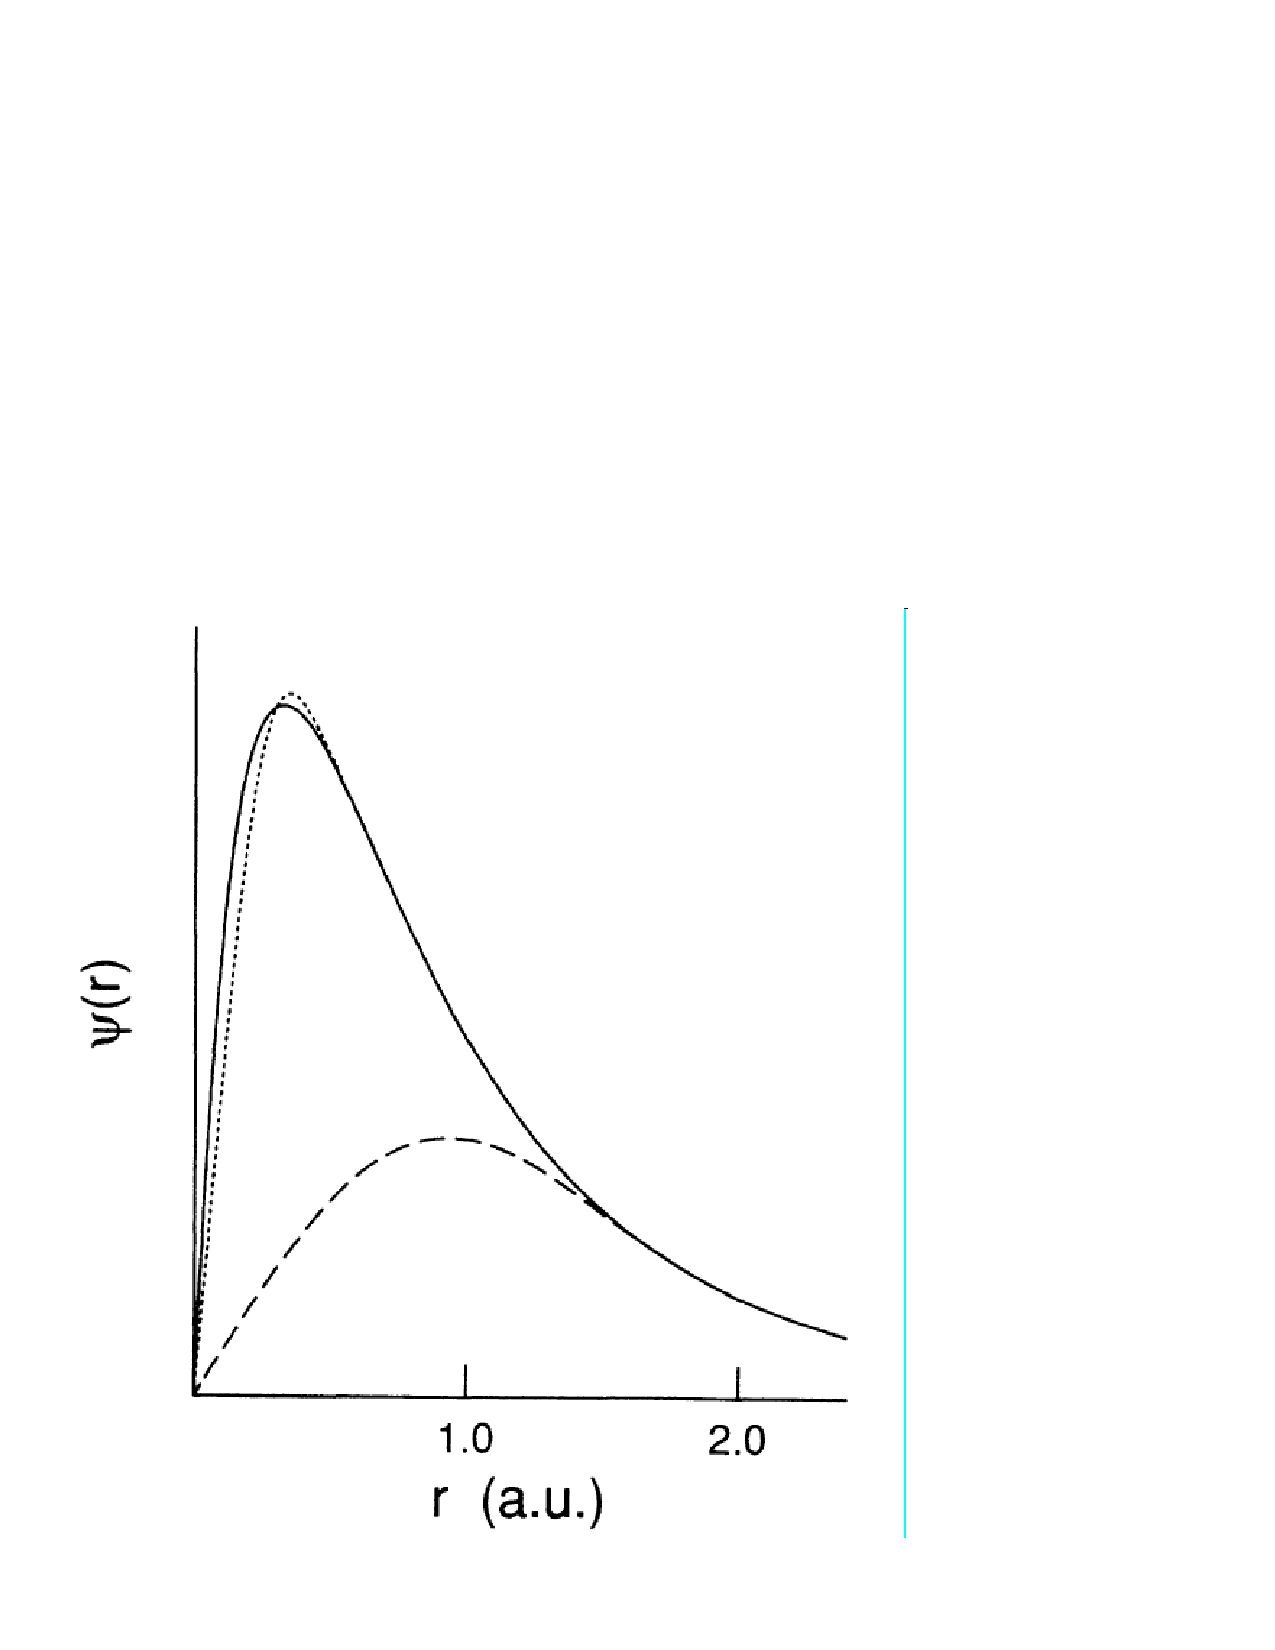
\includegraphics[height=1.35in,width=1.40in,viewport=30 55 415 500,clip]{Figures/Norm-US-wave.pdf}
\caption{\tiny \textrm{Oxygen 2} \textit{p} \textrm{radical wave function (solid), NC-pseudo-wave (dotted) and US-pseudo-wave (dashed).}}%(与文献\cite{EPJB33-47_2003}图1对比)
\label{Norm-US-wave}
\end{figure}
}

\frame
{
	\frametitle{从模守恒赝势到超软赝势}
	为提高模守恒赝势的可移植性\footnote{\tiny{换言之,提升赝波函数能适应的能量变分空间}},\textrm{Vanderbilt}和\textrm{Bl\"ochl}分别建议:\\
	在构造可分离赝势时,\textcolor{blue}{引入额外的参考能量$\varepsilon_l$,并要求对每个角动量量子数$l$,所有能量参数$\varepsilon_l$构造的赝波函数$\phi_i^{\mathrm{ps}}$及其辅助函数$\chi_i$都满足
	\begin{displaymath}
		|\chi_i\rangle=-(\mathbf{T}+V_{\mathrm{loc}}-\varepsilon)|\phi_i^{\mathrm{ps}}\rangle
	\end{displaymath}}
	{\fontsize{7.2pt}{5.2pt}\selectfont{这里$i$表示量子数$l$,$m$和能量参数$\varepsilon$,即$i=(lm,\varepsilon)$}}
	\vskip 5pt
	由此出发,可构造出一组与赝波函数$\phi_i^{\mathrm{ps}}$垂直的函数$\beta_i$:~
{\fontsize{7.2pt}{5.2pt}\selectfont{
	\begin{itemize}
		\item 构造矩阵$\mathbf{B}$,其矩阵元$B_{ij}$满足
			\begin{displaymath}
				B_{ij}= \langle\phi_j^{\mathrm{ps}}|\chi_i\rangle
			\end{displaymath}
		\item 由矩阵$\mathbf{B}$和$\chi$得到函数$\beta_i$
			\begin{displaymath}
				|\beta_i\rangle=\sum_j(\mathbf{B}^{-1})_{ij}|\chi_j\rangle
			\end{displaymath}
		\item 由此得到的$\beta$与赝波函数$\phi_i^{\mathrm{ps}}$满足正交条件
	\begin{displaymath}
		\langle\beta_i|\phi_j^{\mathrm{ps}}\rangle=\delta_{ij}
	\end{displaymath}
	\end{itemize}}}
}

\frame
{
	\frametitle{从模守恒赝势到超软赝势}
	因此可分离赝势的非局域部分表示为
	\textcolor{blue}{\begin{displaymath}
		V_{\mathrm{NL}}=\sum_i|\chi_i\rangle\langle\beta_i|=\sum_{ij}B_{ij}|\beta_j\rangle\langle\beta_i|
	\end{displaymath}}
	{\fontsize{7.2pt}{5.2pt}\selectfont{不难看出,如果赝波函数满足广义模守恒条件
	\begin{displaymath}
		Q_{ij}=\langle\phi_j^{\mathrm{AE}}|\phi_i^{\mathrm{AE}}\rangle-\langle\phi_j^{\mathrm{PS}}|\phi_i^{\mathrm{PS}}\rangle = 0
	\end{displaymath}
	亦即
	\begin{displaymath}
		Q_{l\varepsilon,l\varepsilon^{\prime}}=\int_0^{R_c}\bigg(\phi_{l\varepsilon}^{\mathrm{AE}}(r)\phi_{l\epsilon^{\prime}}^{\mathrm{AE}}(r)-\phi_{l\varepsilon}^{\mathrm{PS}}(r)\phi_{l\varepsilon^{\prime}}^{\mathrm{PS}}(r)\bigg)\mathrm{d}r=0
	\end{displaymath}
	将大大提高赝势的可移植性。
	\vskip 5pt
	但实际上,广义模守恒条件看似简单,当能量参数$\varepsilon\neq\varepsilon^{\prime}$,要满足这个条件
	$$Q_{l\varepsilon,l\varepsilon^{\prime}}=0$$
	并非易事;~而一旦模守恒条件被破坏,矩阵$\mathbf{B}$(相应地,赝势的非局域部分$V_{\mathrm{NL}}$)就是非\textrm{Hermitian}}}
}

\frame
{
\frametitle{超软赝势的构造}
\textrm{Vanderbilt}建议构造赝波函数时放弃模守恒约束条件,只要求价电子赝波函数与真实电子波函数的径向部分在截断半径$r_{c,l}$外相同,由此得到的赝势显然非\textrm{Hermitian},但是通过构造\\\textcolor{blue}{\textrm{Hermitian}重叠算符}
\begin{displaymath}
	\mathbf{S}=\mathbf{1}+\sum_{i,j}Q_{ij}|\beta_j\rangle\langle\beta_i|
\end{displaymath}
以及\textcolor{blue}{\textrm{Hermitian}赝势算符}
\begin{displaymath}
	\tilde V^{\mathrm{NL}}=\sum_{i,j}\mathbf{D}_{i,j}|\beta_j\rangle\langle\beta_i|
\end{displaymath}
这里\textcolor{blue}{
\begin{displaymath}
	\mathbf{D}_{ij}=B_{ij}+\varepsilon_iQ_{ij}
\end{displaymath}}
模守恒约束下的标准本征值方程将变成广义本征值方程
\begin{displaymath}
	(T+V_{\mathrm{loc}}+\tilde V^{\mathrm{NL}}-\varepsilon\mathbf{S})|\phi\rangle=0
\end{displaymath}
}

\frame
{
\frametitle{超软赝势的特点}
\textrm{Vanderbilt}的超软赝势构造方案最大的优点是
\begin{itemize}
	\item \textcolor{purple}{解除模守恒约束}:~有助于增加赝波函数的截断半径,系统提高赝势的柔软程度
	\item \textcolor{purple}{引入多个参考能量$\varepsilon_l$}:~使得模守恒条件下只在特定参考能量$\varepsilon$处成立的对数导数连续条件,扩展到参考能量$\varepsilon_l$区间范围内,这大大提高了赝势的适用范围(可移植性)
\end{itemize}

相应的,超软赝势计算中,电子密度表达形式为
\begin{displaymath}
	n(r)=\sum_nf_n|\phi_n(r)|^2+\sum_{n,ij}f_n\langle\phi_n|\beta_j\rangle\langle\beta_i|\phi_n\rangle Q_{ij}(r)
\end{displaymath}
这里补偿电荷$Q_{ij}(r)$定义为
\begin{displaymath}
	Q_{ij}(r)=\phi_i^{\mathrm{AE}}(r)\phi_j^{\mathrm{AE}}(r)^{\ast}-\phi_i^{\mathrm{US}}(r)\phi_j^{\mathrm{US}}(r)^{\ast}
\end{displaymath}
}

\frame
{
\frametitle{补偿电荷与多极矩}
根据电动力学定理:\\\textcolor{blue}{如果球\textrm{S}内的电荷密度分布$\rho(\vec r)$,在球外某点$\vec r$产生的势是由电荷密度的多极矩确定}:
\begin{figure}[h!]
\vspace*{-15pt}
\centering
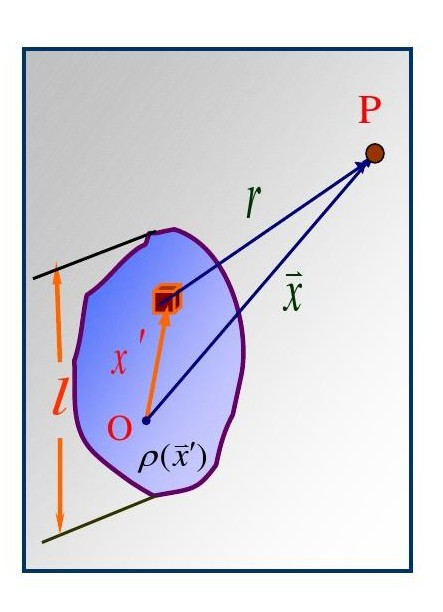
\includegraphics[height=1.25in,width=1.32in,viewport=1 22 507 575,clip]{Figures/potential_multipole.jpg}
%\caption{\tiny \textrm{From Muffin-tin Potential to Full Potential}}%(与文献\cite{EPJB33-47_2003}图1对比)
\label{Potential-multipole}
\end{figure}
\begin{displaymath}
	V(\vec r)=\sum_{l=0}^{\infty}\sum_{m=-l}^{l}\dfrac{4\pi}{2l+1}q_{lm}\dfrac{Y_{lm}(\hat{\vec r})}{r^{l+1}}
\end{displaymath}
其中多极矩$q_{lm}$由下式计算
\begin{displaymath}
	q_{lm}=\int_SY_{lm}^{\ast}(\hat{\vec r})r^l\rho(\vec r)\mathrm{d}^3r
\end{displaymath}
}

\frame
{
	\frametitle{\textrm{US-PP}的总能量表示}
	根据\textrm{D. Vanderbilt}的超软赝势(\textrm{US-PP})方案
	原子波函数满足$$(T+V_{\mathrm{AE}}-\varepsilon_n)|\psi_n\rangle=0$$
	据此构造原子赝波函数$\phi_n$,在截断半径$r_c^l$处,$\phi_n$与$\psi_n$平滑衔接(不需要模守恒条件)

	类似地,构造局域平滑势$V_{loc}(r)$,在截断半径$r_c^{loc}$处,$V_{loc}(r)$与$V_{\mathrm{AE}}(r)$平滑衔接
	
	构造辅助轨道
	$$|\chi_n\rangle=(\varepsilon_n-T-V_{loc})|\phi_n\rangle$$
	由此构造内积矩阵,矩阵元$$B_{nm}=\langle\phi_n|\chi_m\rangle$$
	并有$$|\beta_n\rangle=\sum_m(B^{-1})_{mn}|\chi_m\rangle$$
	这里$\beta_n$是局域函数,并与$\phi_n$垂直
}

\frame
{
	\frametitle{\textrm{US-PP}的总能量表示}
	定义\textcolor{orange}{缀加函数}$$Q_{nm}(\vec r)=\psi_n^{\ast}(\vec r)\psi_m(\vec r)-\phi_n^{\ast}(\vec r)\phi_m(\vec r)$$
	\textcolor{blue}{可赝化的补偿电荷}$$q_{nm}=\langle\psi_n|\psi_m\rangle_R-\langle\phi_n|\phi_m\rangle_R$$
	由此可以导出$\phi_n$满足久期方程
	\begin{displaymath}
		\begin{aligned}
			&\left(T+V_{loc}+\sum_{nm}D_{nm}|\beta_n\rangle\langle\beta_m|\right)|\phi_n\rangle\\
			=&\varepsilon_n\left(1+\sum_{nm}q_{nm}|\beta_n\rangle\langle\beta_m|\right)|\phi_n\rangle
		\end{aligned}
	\end{displaymath}
	其中$$D_{nm}=B_{nm}+\varepsilon_nq_{nm}$$
}

\frame
{
	\frametitle{\textrm{US-PP}的总能量表示}
	在超软赝势方法中,包含$N_v$个价电子体系的总能量\upcite{PRB47-10142_1993}
	\begin{displaymath}
		\begin{aligned}
			E_{\mathrm{tot}}[\{\phi_i\},\{\vec R_I\}]=&\sum_i\langle\phi_i|-\frac12\nabla^2+V_{\mathrm{NL}}|\phi_i\rangle\\
			&+\frac12\iint\mathrm{d}\vec r\mathrm{d}\vec r\,^{\prime}\dfrac{n(\vec r)n(\vec r\,^{\prime})}{|\vec r-\vec r\,^{\prime}|}\\
			&+\int\mathrm{d}\vec r V_{loc}^{\mathrm{ion}}(\vec r)n(\vec r)+E_{\mathrm{XC}}[n]\\
			&+U(\{\vec R_I\})
		\end{aligned}
	\end{displaymath}
	这里$\phi$是体系波函数,$n(\vec r)$是电子密度,$E_{\mathrm{XC}}$是交换-相关能,$U(\{\vec R_I\})$是离子-离子相互作用能
}

\frame
{
	\frametitle{\textrm{US-PP}的总能量表示}
	电荷密度$$n(\vec r)=\sum_i\big[|\phi_i(\vec r)|^2+\sum_{nm,I}Q_{nm}^I(\vec r)\langle\phi_i|\beta_n^I\rangle\langle\beta_m^I|\phi_i\rangle\big]$$
	局域势$$V_{loc}^{\mathrm{ion}}(\vec r)=\sum_IV_{loc}^{\mathrm{ion}}(\vec r-\vec R_I)$$
	$V_{loc}^{\mathrm{ion}}$由$V_{loc}$去屏蔽后得到$$V_{loc}^{\mathrm{ion}}(r)=V_{loc}(r)-\int\mathrm{d}\vec r\,^{\prime}\dfrac{n(\vec r\,^{\prime})}{|\vec r-\vec r\,^{\prime}|}-\mu_{\mathrm{XC}}(r)$$
	非局域部分$$V_{\mathrm{NL}}=\sum_{nm,I}D_{nm}^{(0)}|\beta_n^I\rangle\langle\beta_m^I|$$
	这里$$D_{nm}^{(0)}=D_{nm}-\int\mathrm{d}\vec r\,^{\prime}V_{loc}(\vec r\,^{\prime})n(\vec r\,^{\prime})$$
}

\frame
{
	\frametitle{超软赝势总能量计算}
	去除价电子屏蔽效应的贡献后,可得最终超软赝势的总能量表达式
	\begin{displaymath}
		\begin{aligned}
			E_{\mathrm{total}}=&\sum_j^{\mathrm{occ}}\langle\phi_{lmj}|\bigg[-\dfrac12\nabla^2+V_{\mathrm{local}}^{\mathrm{ion}}+\sum_{s,s^{\prime}}\mathbf{D}_{s,s^{\prime}}^{\mathrm{ion}}|\beta_s\rangle\langle\beta_{s^{\prime}}|\bigg]|\phi_{lmj}\rangle\\
			&+E_{H}[n_v]+E_{N-N}+E_{XC}[n_v]
		\end{aligned}
	\end{displaymath}
	{\fontsize{7.2pt}{5.2pt}\selectfont{其中$n_v(r)=\sum\limits_j^{\mathrm{occ}}\phi_{lmj}^{\ast}(r)\phi_{lmj}(r)+\sum\limits_{s,s^{\prime}}\sum\limits_j^{\mathrm{occ}}\langle\phi_{lmj}|\beta_{s^{\prime}}\rangle\langle\beta_s|\phi_{lmj}\rangle Q_{s,s^{\prime}}(r)$
	$$V_{\mathrm{local}}^{\mathrm{ion}}=V_{\mathrm{local}}-V_{\mathrm H}-V_{XC}$$
	$$\mathbf{D}_{s,s^{\prime}}^{\mathrm{ion}}=\mathbf{D}_{s,s^{\prime}}-\int\mathrm{d}\vec r\big[V_{\mathrm{H}}(\vec r)+V_{XC}(\vec r)\big]Q_{s,s^{\prime}}(r)$$}}
	由此可得超软赝势的广义本征值方程
	$$\bigg[-\dfrac12\nabla^2+V_{\mathrm{local}}+\tilde V_{NL}^{\mathrm{US}}-\varepsilon_i\bigg(\mathbf{1}+\sum_{s,s^{\prime}}Q_{s,s^{\prime}}|\beta_s\rangle\langle\beta_{s^{\prime}}|\bigg)\bigg]|\phi_{lmi}\rangle=0$$
}

\subsection{赝势方法与\rm{PAW}方法}
\frame
{
%	\frametitle{\textrm{PAW}原子数据集}
	\frametitle{\textrm{PAW Augmentation}}
\begin{figure}[h!]
\centering
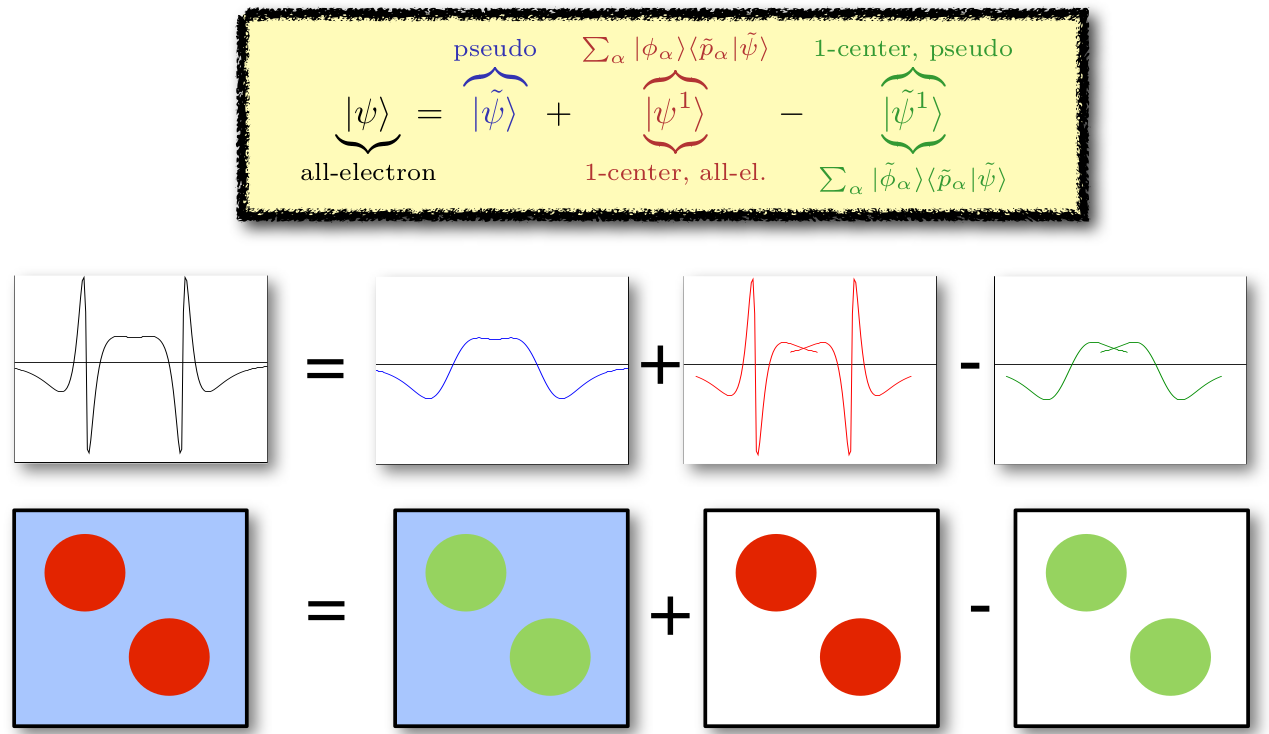
\includegraphics[height=2.3in,width=4.0in,viewport=0 0 1280 745,clip]{Figures/PAW-baseset.png}
\caption{\tiny \textrm{The Augmentation of PAW.}}%(与文献\cite{EPJB33-47_2003}图1对比)
\label{PAW_baseset}
\end{figure}
}

\frame
{
\frametitle{电荷密度的重新分解}
\textrm{PAW}方法提出后有很长一段时间没有能够得到广泛应用,直到\textrm{G. Kresse}等将\textrm{Bl\"ochl}的原始方案中电荷密度计算方案重新组合后,明确了\textrm{PAW}方法与\textrm{USPP}方法的内在联系。
\begin{itemize}
	\item 芯层电荷与核电荷构成离子实电荷:$n_{Zc}=n_Z+n_c$
\end{itemize}
\begin{figure}[h!]
\centering
\vspace{-10.5pt}
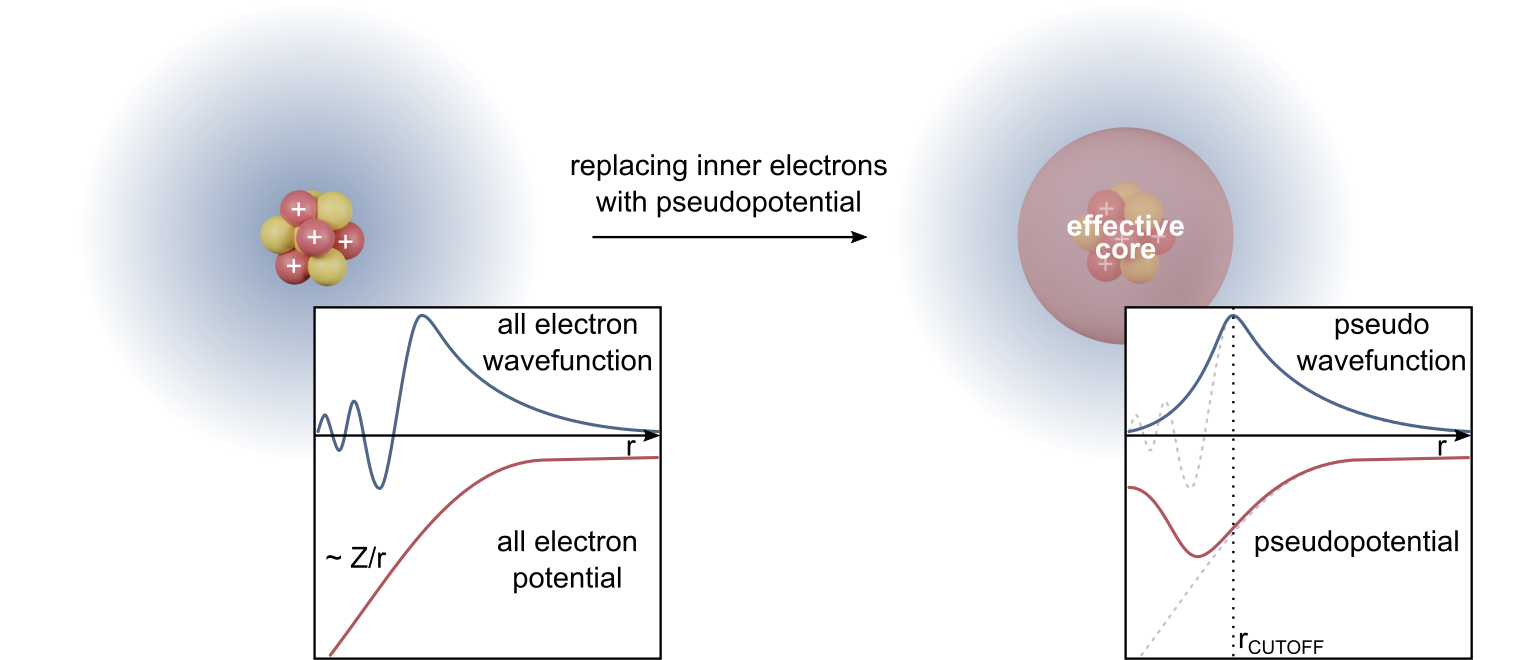
\includegraphics[height=1.5in,width=3.0in,viewport=0 0 380 190,clip]{Figures/Pseudo-potential_charge.png}
\caption{\tiny \textrm{The difference of the electron-density distributing from P.~Bl\"ochl  and from G.~Kresse.}}%(与文献\cite{EPJB33-47_2003}图1对比)
\label{PAW_Pseudo-Charge}
\end{figure}
}

\frame
{
	\frametitle{电荷密度重新分解与赝势}
\begin{itemize}
	\item 构造赝离子实电荷$$\int_{\Omega_c}n_{Zc}(\vec r)\mathrm{d}^3\vec r=\int_{\Omega_c}\tilde n_{Zc}(\vec r)\mathrm{d}^3\vec r$$
\end{itemize}
在此基础上,\textrm{Bl\"ochl}方案中的电荷可以分解为:
\begin{displaymath}
	\begin{aligned}
		n_T=n+n_{Zc}\equiv&\underbrace{(\tilde n+\hat n+\tilde n_{Zc})}\\
				 		&\quad\qquad\tilde n_T\\
				  &+\underbrace{(n^1+\hat n+n_{Zc})}-\underbrace{(\tilde n^1+\hat n+\tilde n_{Zc})}\\
				                  &\quad\qquad n_T^1\qquad\qquad\qquad\tilde n_T^1
	\end{aligned}
\end{displaymath}
\textcolor{red}{注意}:\textrm{G. Kresse}方案中补偿电荷$\hat n$局域在每个缀加球内。
}

\frame
{
	\frametitle{\textrm{Hartree~}势的分解}
\begin{displaymath}
	\begin{aligned}
		\dfrac12(n_T)(n_T)=&\dfrac12(\tilde n_T)(\tilde n_T)+(n_T^1-\tilde n_T^1)(\tilde n_T)\\
				&+\dfrac12(n_T^1-\tilde n_T^1)(n_T^1-\tilde n_T)
	\end{aligned}
\end{displaymath}
这里$$(a)(b)=\int\mathrm{d}\vec r\mathrm{d}\vec r^{\prime}\dfrac{a(\vec r)b(\vec r\,^{\prime})}{|\vec r-\vec r\,^{\prime}|}$$
\textcolor{red}{近似}:$\tilde n_T$用$\tilde n_T^1$替换:
\begin{displaymath}
	\dfrac12(n_T)(n_T)=\dfrac12(\tilde n_T)(\tilde n_T)-\dfrac12\overline{(n_T^1(\tilde n_T^1)}+\dfrac12\overline{(n_T^1)(n_T^1)}
\end{displaymath}
}

\frame
{
\frametitle{交换-相关能泛函的处理}
由于交换-相关能泛函是非线性的,\textrm{G. Kresse}方案中电荷密度分解为
\begin{displaymath}
	n_c+n=(\tilde n+\hat n+\tilde n_c)+(n^1+n_c)-(\tilde n^1+\hat n+\tilde n_c)
\end{displaymath}
原始的\textrm{Bl\"ochl}方案中电荷分解为
\begin{displaymath}
	n_c+n=(\tilde n)+(n^1+n_c)-(\tilde n^1)
\end{displaymath}
\textcolor{blue}{两种不同的电荷密度分解方案根源}:\\\textrm{G. Kresse}方案中赝离子实电荷$\tilde n_{Zc}$与\textrm{Bl\"ochl}方案中$\tilde n_c$的约束条件不同!
\begin{displaymath}
	E_{\mathrm{XC}}[\tilde n+\hat n+\tilde n_c]+\overline{E_{\mathrm{XC}}[n^1+n_c]}-\overline{E_{\mathrm{XC}}[\tilde n^1+\hat n+\tilde n_c]}
\end{displaymath}
}

\subsection{赝势方法与全势方法}
\subsection{\rm{APW~}与\rm{LAPW~}方法}
\frame
{
	\frametitle{\textrm{Muffin-tin}近似}
\begin{figure}[h!]
\centering
\subfigure[\textrm{Muffin-tin Potentional}]{
\label{Semi-local-potential}
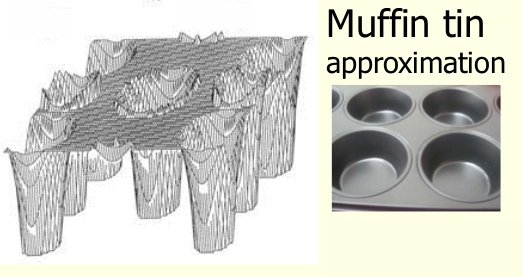
\includegraphics[height=1.10in,width=1.92in,viewport=1 22 507 295,clip]{Figures/Muffin-tin.png}}
\subfigure[\textrm{Division of the unit cell into spheres(I) and into interstitial region(II)}]{
\label{Semi-local-space}
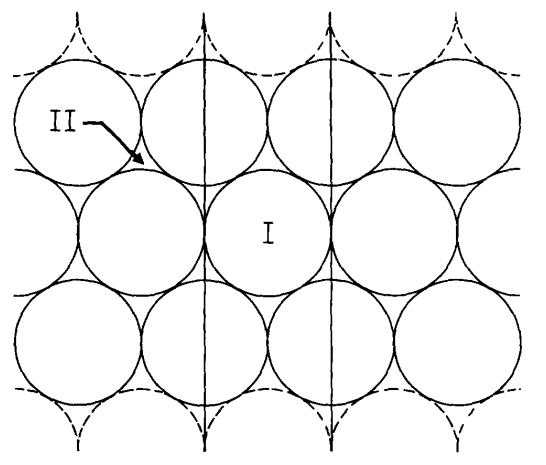
\includegraphics[height=1.45in,width=1.92in,viewport=1 20 515 435,clip]{Figures/Muffin-Tin.png}}
%\caption{\tiny \textrm{Division of the unit cell into spheres(I) and into interstitial region(II)}}%(与文献\cite{EPJB33-47_2003}图1对比)
\label{Muffin_tin-1}
\end{figure}
\textrm{Muffin-tin}近似是\textrm{Johnson}采用$\chi_{\alpha}$方法计算分子体系的交换-相关时,引入多重散射(\textrm{Multiple scattering})理论时提出的%,\textrm{Muffin-tin}直译为“松饼罐头”,意思是把分子中的原子看成堆在一起的圆球罐

\textcolor{red}{\textrm{MT}球近似与多重散射理论有密切的关联}
}

\frame
{
\frametitle{\textrm{APW}方法}
\begin{figure}[h!]
\centering
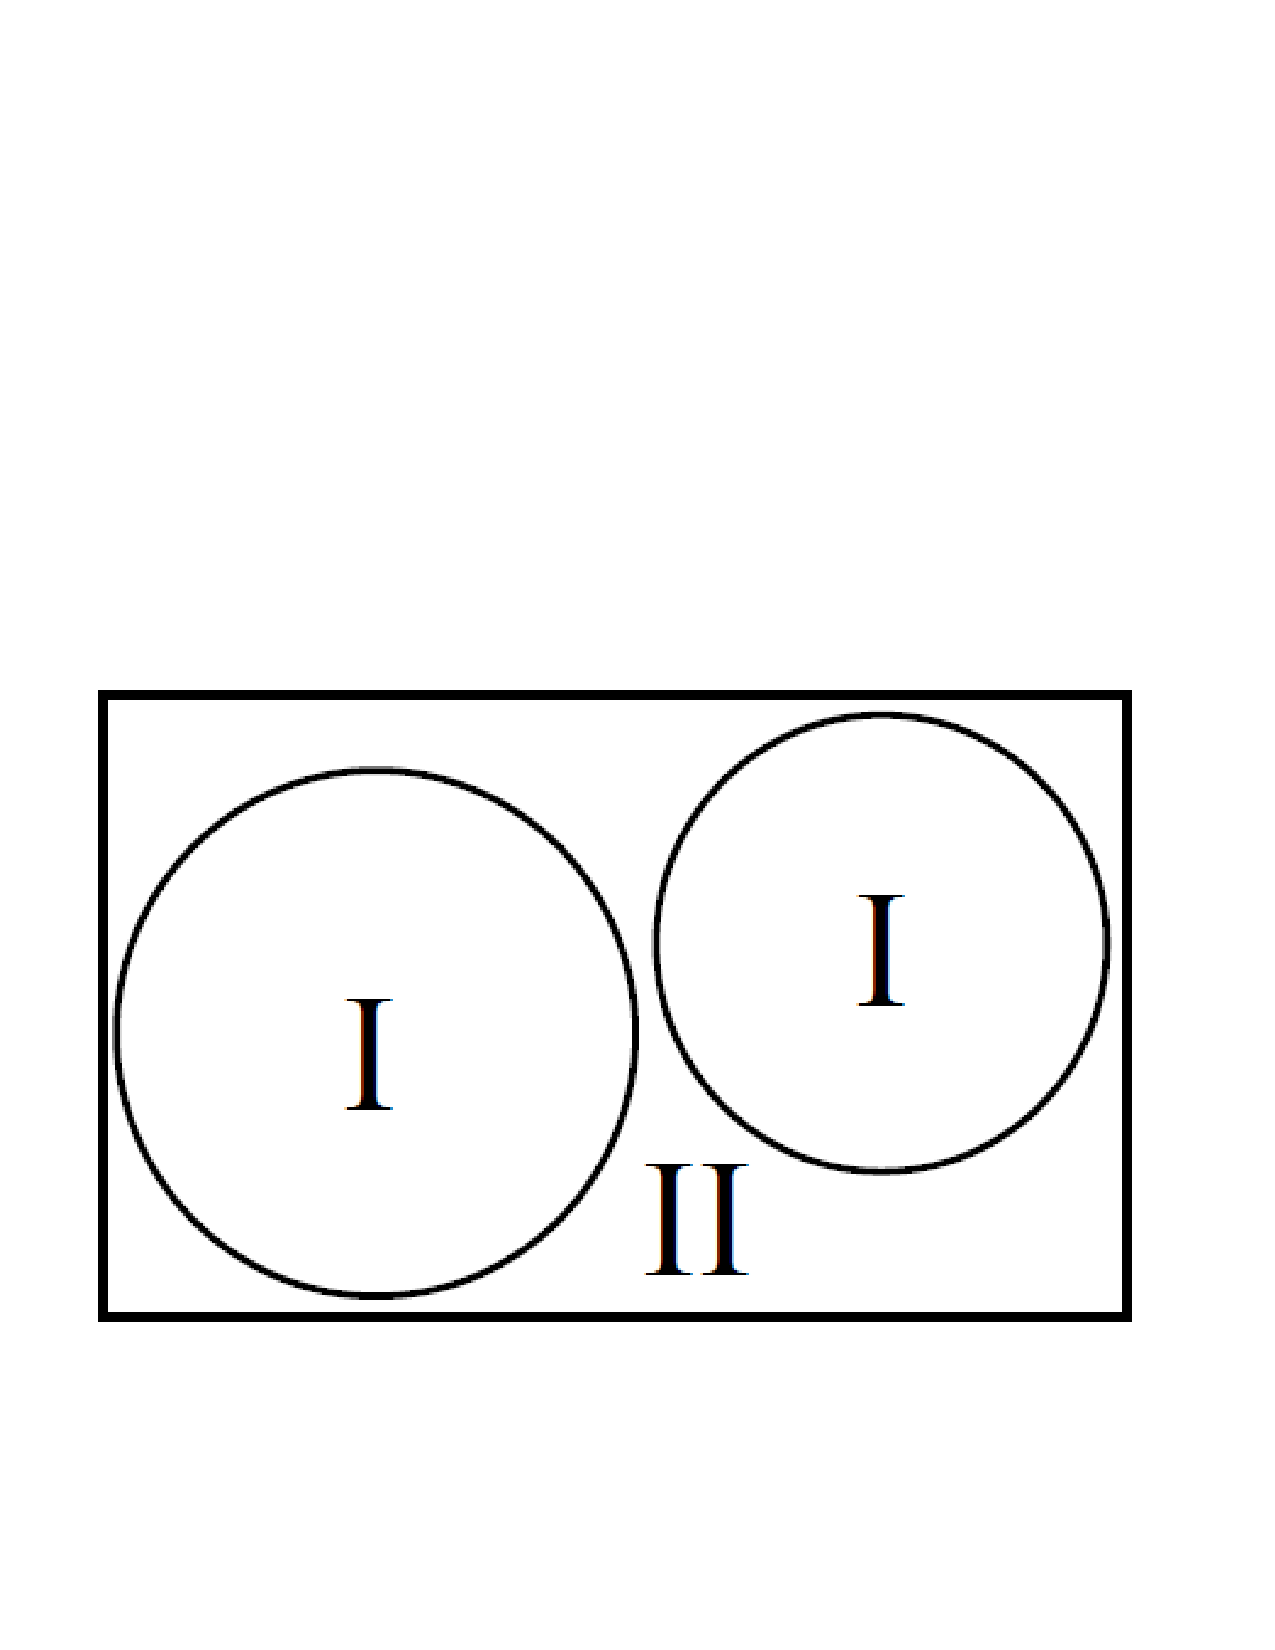
\includegraphics[height=1.10in,width=1.80in,viewport=40 150 545 465,clip]{Figures/Muffin_tin.pdf}
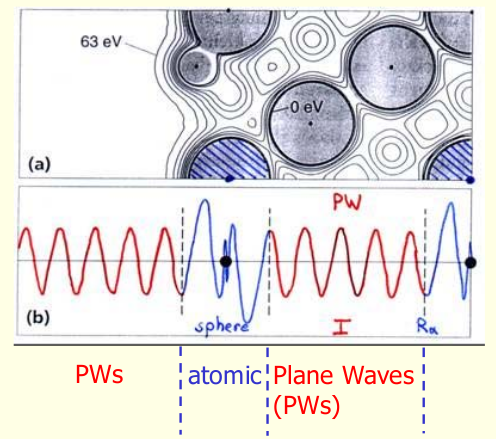
\includegraphics[height=1.10in,width=1.45in,viewport=1 20 485 435,clip]{Figures/APW.png}
\caption{\tiny \textrm{Partitioning of the unit cell into atomic spheres(I) and an interstitial region(II)}}%(与文献\cite{EPJB33-47_2003}图1对比)
\label{Muffin_tin-2}
\end{figure}
\begin{displaymath}
\hskip -28pt\footnotesize \varphi(\vec k_j,\vec r)=\left\{
  \begin{aligned}
    &\Omega^{-1/2}\exp[i\vec k_j\cdot\vec r],&|\vec r-\vec r_s|>R_{\mathrm{MT}}^s\\
    &\sum_{lm}A_{lm}^{\vec k_j}u_l(|\vec r-\vec r_s|,E)Y_{lm}(\widehat{\vec r-\vec r_s}),&|\vec r-\vec r_s|\leqslant R_{\mathrm{MT}}^s
  \end{aligned}
\right.
\end{displaymath}
}

\frame
{
	\frametitle{空间两部分函数在球面上的衔接}
	\textrm{Huygens}原理:~\textcolor{blue}{平面波可以在各个原子球中心用球谐函数展开}:
	\begin{displaymath}
		\mathrm{e}^{\mathrm{i}\vec k\cdot\vec r}=4\pi\sum_{l=0}^{\infty}\sum_{m=-l}^l\mathrm{i}^lj_l(|\vec k|r)Y_{lm}^{\ast}(\hat{\vec k})Y_{lm}(\hat{\vec r})
	\end{displaymath}
	其中$j_l(|\vec k|r)$是$l$-阶球\textrm{Bessel}函数,$\hat{\vec k}$和$\hat{\vec r}$分别是矢量$\vec k$和$\vec r$与直角坐标$z$-轴的夹角$\theta$和$\varphi$

	要求空间中不同区域函数在球面上连续,可调参数$A_{lm}^{\vec k}$可为下式确定
\begin{displaymath}
	A_{lm}^{\vec k}=4\pi\mathrm{e}^{\mathrm{i}\vec k\cdot\vec r_s}\mathrm{i}^lY_{lm}^{\ast}(\hat{\vec k})j_l(|\vec k|R_{MT}^s)/u_l(R_{MT}^s,E)
\end{displaymath}
\textrm{APW}的问题:\textcolor{blue}{球面参数$A_{lm}^{\vec k}$对能量$E$依赖,由此构造的久期方程\footnote{\fontsize{7.2pt}{6.2pt}\selectfont{久期方程\textrm{secular~equation},\textrm{secular}来自拉丁语\textrm{saeculum},本意为一代人、一个时期、一个时代、一个世界等意思。其名词在拉丁语中就作为世纪讲。汉译\textrm{secular}为久期,是取\textrm{long-term}的意思(实为慢,\textrm{slow~in~comparison~to~the~annual~motion}的意思),与期待\textrm{(expectation)}无关\upcite{PhysCN40-477_2011}。}}非线性的}
}

\frame
{
\frametitle{\textrm{LAPW}方法}
%\small\textrm{APW}方法的困难,久期方程不能化成广义本征值方程的形式(久期方程对能量$E$是非线性的)为了克服这一困难,人们提出线性化方法,
\textrm{O.~K.~Andersen~}提出\textrm{LAPW}方法\upcite{Singh}:将$u_l(r,E)$在某一合适的$E_l$值附近对$E$的一阶微商{$\left.\dfrac{\textrm{d}u_l(r,E)}{\textrm{d}E}\right|_{E_l}\equiv\dot u_l(r,E_l)$}\\代入\textrm{APW}基函数中可得\textrm{LAPW}方法的基函数:
{\fontsize{7.5pt}{3.3pt}\selectfont
$$\hskip -14pt \varphi(\vec k_j,\vec r)=\left\{
  \begin{aligned}
    &\Omega^{-1/2}\exp[i\vec k_j\cdot\vec r],&|\vec r-\vec r_s|>R_{\mathrm{MT}}^s\\
    &\sum_{lm}[A^{\vec k_j}_{lm}u_l(|\vec r-\vec r_s|,E_l)+B^{\vec k_j}_{lm}\dot u_l(|\vec r-\vec r_s|,E_l)]Y_{lm}(\widehat{\vec r-\vec r_s}),&|\vec r-\vec r_s|\leqslant R_{\mathrm{MT}}^s
  \end{aligned}
\right.$$
%$$\Psi_{\vec k}(\vec r)=\int_{\Omega}\tilde G_{\vec k}(\vec r-\vec r\,^\prime;E)V(\vec r\,^\prime)\Psi_{\vec k}(\vec r\,^\prime)\textrm{d}\vec r\,^\prime$$
根据基函数在\textrm{MT}球面上连续到一阶,确定系数$A^{\vec k}_{lm}$,$B^{\vec k}_{lm}$的值。}
\begin{figure}[h!]
	\vskip -3pt
\centering
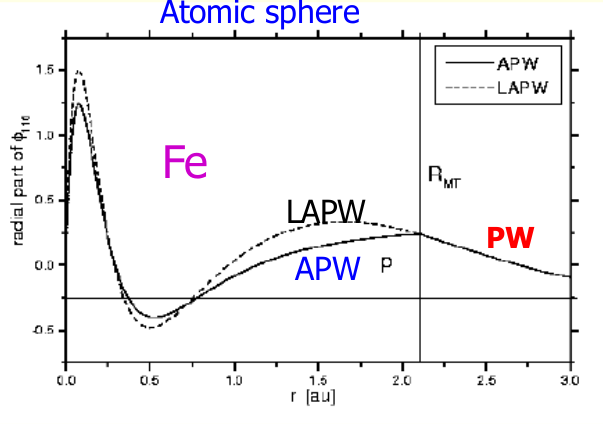
\includegraphics[height=1.10in,width=1.88in,viewport=1 20 585 435,clip]{Figures/WIEN2k-LAPW.png}
\caption{\tiny \textrm{Partitioning of the unit cell into atomic spheres(I) and an interstitial region(II)}}%(与文献\cite{EPJB33-47_2003}图1对比)
\label{Muffin_tin-3}
\end{figure}
}

\subsection{全势的基本思想}
\frame
{
\frametitle{全势的基本思想}
全势\textrm{(Full Potential, FP)}是相对于赝势的概念,即\textcolor{blue}{电子运动过程中感受到其它粒子作用的真实效果}。
实际计算中,构造\textrm{LAPW}基组的\textrm{MT}势换成晶体势函数。一般地,在每个\textrm{MT}球内,势函数用球谐函数(或者是满足晶体对称性)展开,\textrm{MT}球外的势函数用\textrm{Fourier}级数展开:%\upcite{PRB13-5362_1976}
{\footnotesize$$ V(\vec r)=\left\{
  \begin{aligned}
    &\sum_{a,L}V_L^a(r)Y_L(\hat{\vec r})\quad &r\leqslant R_{\mathrm{MT}}^a\\
    &\sum_{\vec G_n}V_I(\vec G_n)\textrm{e}^{i\vec G_n\cdot\vec r} &\vec r\in\mathrm{II}
  \end{aligned}\right.
  \label{eq:solid-63}
$$}
这里$L$\,$\equiv$\,$l,m$,$\vec G_n$为倒格矢,$Y_L(\hat{\vec r})$是球谐函数,\textrm{II}为原子间隙
\begin{itemize}
	\item 在\textrm{MT}球内靠近原子核,势能具有原子型势能特征
	\item 在\textrm{MT}球外,要满足\textrm{Bloch}函数边界条件特征。
	\item 在\textrm{MT}球内外的势能表象不同,同样要求势能在\textrm{MT}球表面连续。
\end{itemize}
}

\frame
{
	\frametitle{全势方法在$\vec k$空间的实现}
\textrm{Weiner}提出全势计算的实现方法\upcite{JMP22-2433_1981}:~\\
\begin{itemize}
	\item 将\textrm{MT}球外的电荷密度$\rho_I(\vec r)$扩展到球内
	\begin{tikzpicture}[remember picture,overlay]
	\node[xshift=-1.5cm,yshift=1.0cm] at (current page.east) {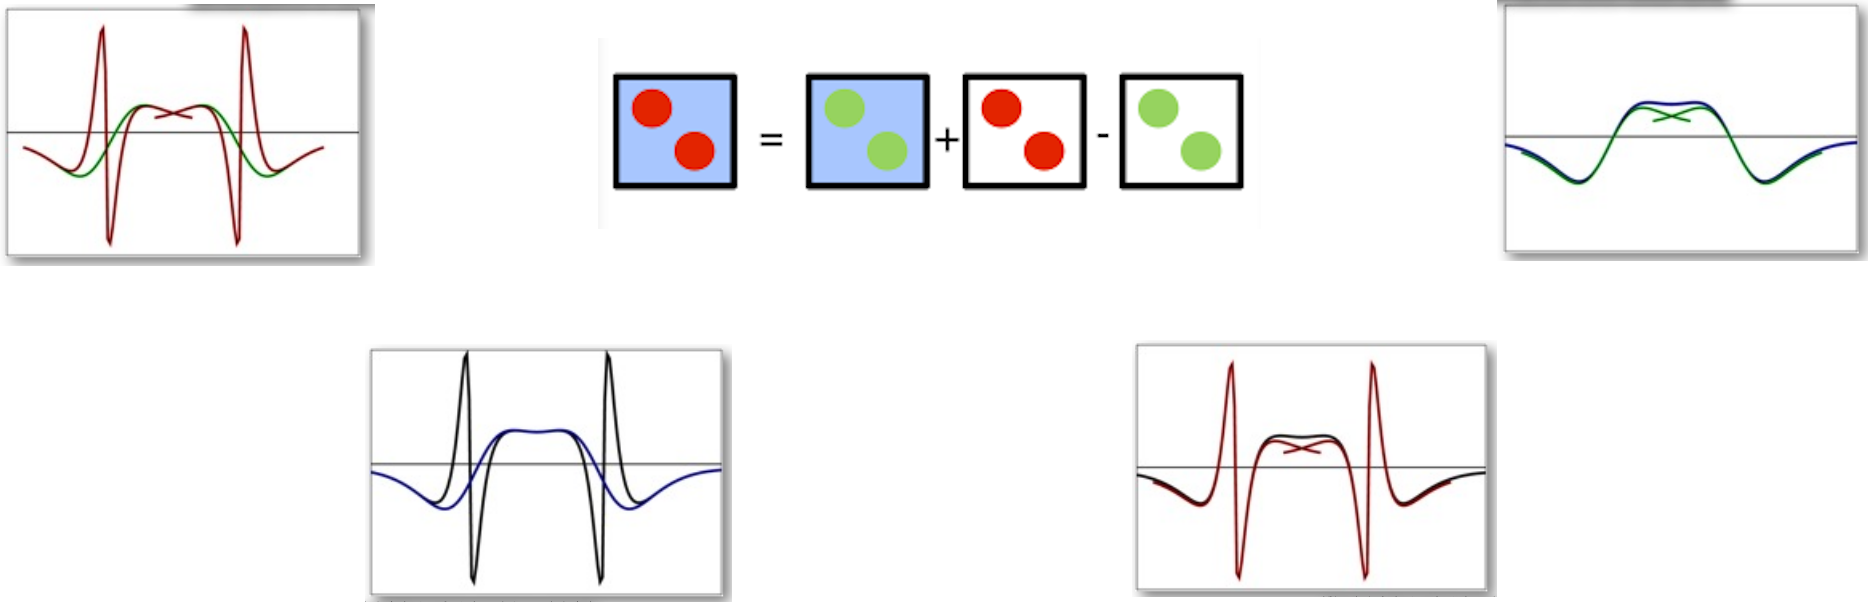
\includegraphics[height=1.7cm, width=2.10cm, viewport=0 340 377 602,clip]{Figures/Full_Potential.png}};
	\end{tikzpicture}
	\begin{displaymath}
		\rho_I(\vec r)=\sum_{\vec K}\rho_I(\vec K)\mathrm{e}^{\mathrm{i}\vec K\cdot\vec r_s}\mathrm{e}^{\mathrm{i}\vec K\cdot(\vec r-\vec r_s)}
	\end{displaymath}
	这部分电荷在每个球内的多极矩展开$q_{lm}^{s,PW}$
	\begin{displaymath}
		\begin{aligned}
			q_{lm}^{s,PW}=&\dfrac{\sqrt{4\pi}}3{R_{MT}^s}^3\rho_I^{(\vec K=0)}\delta_{l0}+\sum_{\vec K\neq0}4\pi\mathrm{i}^l\rho_I(\vec K){R_{MT}^s}^{l+3}\\
			&\times\dfrac{j_{l+1}(|\vec K|R_{MT}^s)}{\vec K\cdot\vec R_{MT}^s}\mathrm{e}^{\mathrm{i}\vec K\cdot\vec r_s}Y_{lm}^{\ast}(\hat{\vec K})
		\end{aligned}
	\end{displaymath}
\end{itemize}
}

\frame
{
	\frametitle{全势方法在$\vec k$空间的实现}
\begin{itemize}
	\item 根据\textrm{MT}球内的电荷密度分布,电子密度$\rho_s(\vec r)$在正空间分布的多极矩$q_{lm}^{s,MT}$
\begin{displaymath}
	q_{lm}^{s,MT}=\int_0^{R_{MT}^s}Y_{lm}^{\ast}(\hat{\vec r})r^l\rho_s(\vec r)\mathrm{d}^3r
\end{displaymath}
由此得到在\textrm{MT}球内,真实电荷密度多极展开多极矩与延伸到球内的平面波电荷多极矩之差
	\begin{displaymath}
		\delta q_{lm}^{s,MT}=q_{lm}^{s,MT}-q_{lm}^{s,PW}
	\end{displaymath}
\begin{figure}[h!]
\centering
\vspace*{-0.05in}
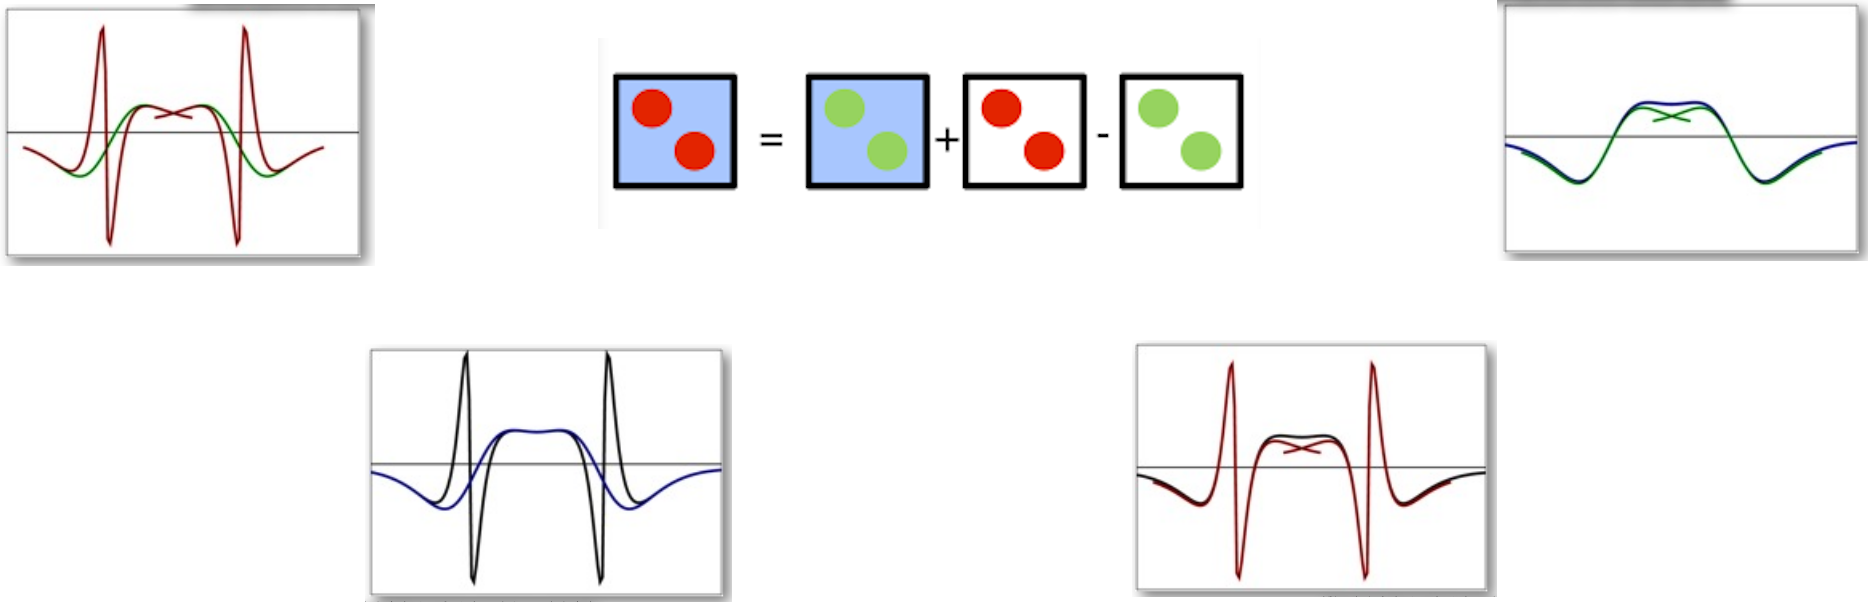
\includegraphics[height=1.00in,width=2.00in,viewport=960 400 1245 540,clip]{Figures/Full_Potential.png}
\caption{\fontsize{4.5pt}{3.2pt}\selectfont{\textrm{The difference of multipole in the sphere.}}}%(与文献\cite{EPJB33-47_2003}图1对比)
\label{Multipol_in-sphere}
\end{figure}
\end{itemize}
}

\frame
{
	\frametitle{全势方法在$\vec k$空间的实现}
\begin{itemize}
	\item 构造赝电荷密度$\tilde\rho(\vec r)$,要求$\tilde\rho(\vec r)$在空间分布平缓,其多级矩$\tilde q_{lm}^{s,MT}$\textcolor{red}{即为$\delta q_{MT}^s$},由此得到赝电荷密度的\textrm{Flourier}变换为
	\begin{displaymath}
		\begin{aligned}
			\tilde\rho_s(\vec K)=&\dfrac{4\pi}{\Omega}\sum_{lm,s}(-\mathrm{i})^l\left\{\dfrac{(-1)^n\tilde q_{lm}^{s,MT}}{2^nn!a_n{R_{MT}^s}^{2l+2n+3}}\dfrac{(2l+2n+3)!!}{(2l+1)!!}\right\}\\
			&\times\left\{(-1)^n2^nn!a_n{R_{MT}^s}^{l+2n+3}\dfrac{j_{l+n+1}(|\vec K|R_{MT}^s)}{(\vec K\cdot\vec R_{MT}^s)^{n+1}}\right\}\\
			&\times\mathrm{e}^{\mathrm{-i}\vec K\cdot\vec r_s}Y_{lm}^{\ast}(\hat{\vec K})
		\end{aligned}
	\end{displaymath}
	\fontsize{6.5pt}{4.2pt}\selectfont{这里$a_n$满足
	\begin{displaymath}
		\sum_{\eta=\nu}^n\dfrac{a_n\eta!R_i^{2\eta}}{(\eta-\nu)!}=0,\qquad \nu=0,1,\cdots,n-1
	\end{displaymath}
	相应的解为
	$a_{\eta}=(-1)^{n-\eta}R_l^{2(n-\eta)}
	\begin{pmatrix}
		n\\\eta
	\end{pmatrix}
	a_n$

%	特殊地,
	当$\vec K=0$时,有
%	\begin{displaymath}
		$\tilde\rho_s(\vec K=0)=\dfrac{\sqrt{4\pi}}{\Omega}\sum\limits_i\tilde{q}_{00}^i$
%	\end{displaymath}
}
\end{itemize}
}

\frame
{
	\frametitle{全势方法在$\vec k$空间的实现}
\begin{itemize}
	\item 在$\vec k$空间内,用平面波电荷密度$\rho_I(\vec K)$叠加\textrm{MT}球内赝电荷密度$\tilde\rho_s(\vec K)$:
		\begin{displaymath}
			\tilde\rho(\vec K)=\tilde\rho_s(\vec K)+\rho_I(\vec K)
		\end{displaymath}
		\textcolor{blue}{这样构造的赝电荷密度,在\textrm{MT}球外产生的势与真实电荷密度分布产生的势相等}
\begin{figure}[h!]
\centering
\vspace*{-0.05in}
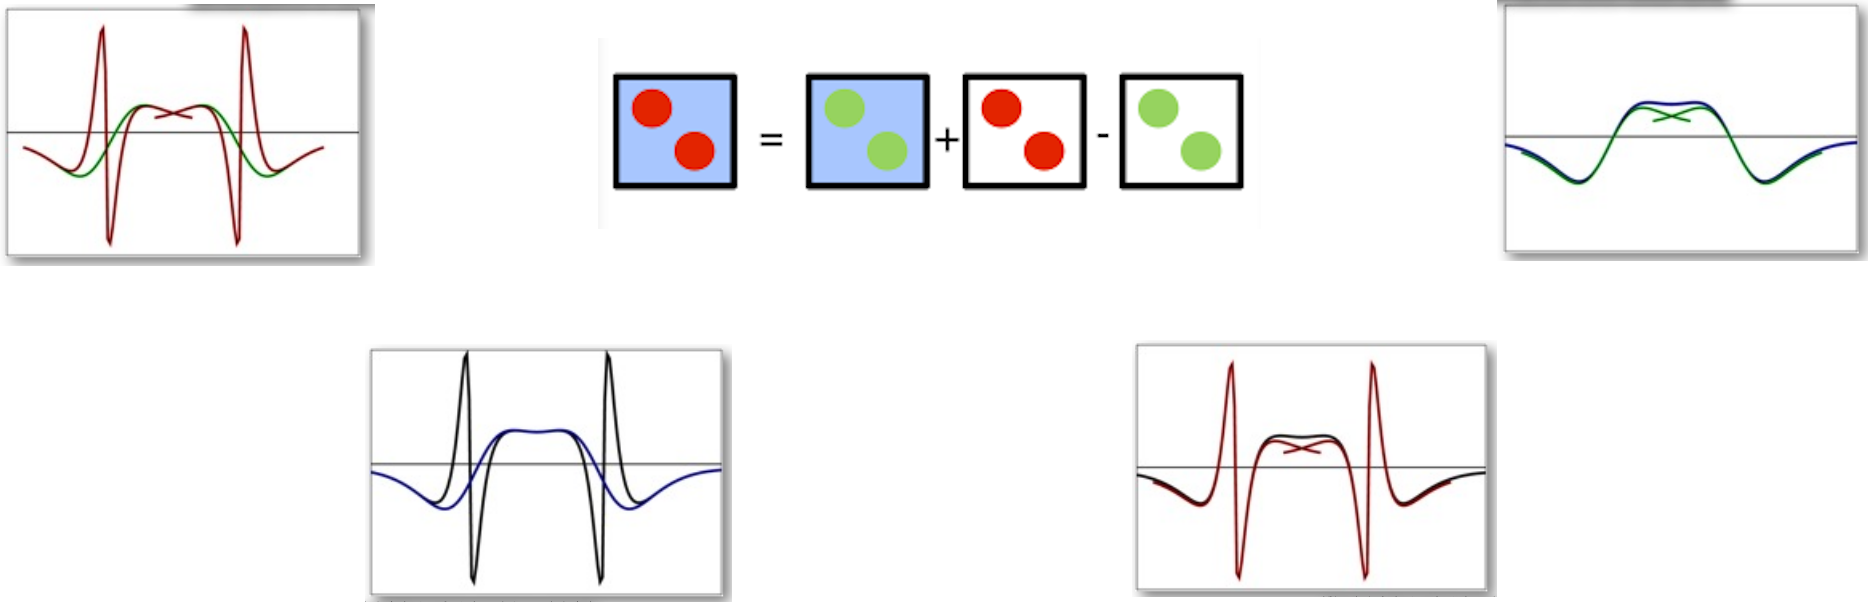
\includegraphics[height=0.60in,width=2.50in,viewport=600 400 1245 540,clip]{Figures/Full_Potential.png}
%\hskip 5pt
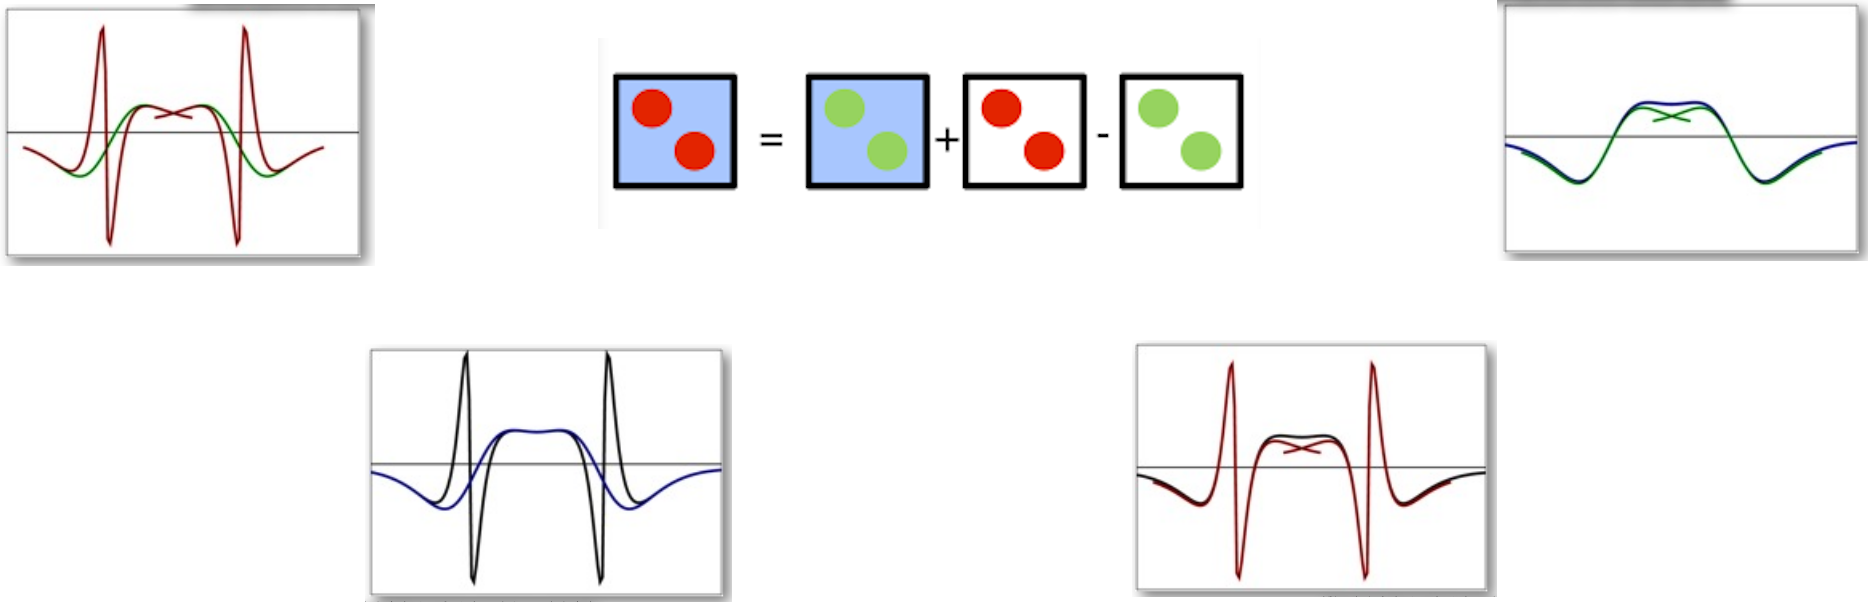
\includegraphics[height=0.70in,width=1.00in,viewport=1480 340 1868 602,clip]{Figures/Full_Potential.png}
\caption{\fontsize{4.5pt}{3.2pt}\selectfont{\textrm{The pseudo charge density for the potential in interstitial zone.}}}%(与文献\cite{EPJB33-47_2003}图1对比)
\label{Pseudo-charge}
\end{figure}
		\fontsize{6.5pt}{4.2pt}\selectfont{根据\textrm{Coulomb}定理计算得到\textrm{Coulomb}势在间隙区的表达式$V_I(\vec K)$(\textrm{Poisson}方程)
		\begin{displaymath}
			V_I(\vec K)=\dfrac{4\pi\tilde\rho(\vec K)}{|\vec K|^2}
		\end{displaymath}}
\end{itemize}
}

\frame
{
	\frametitle{全势方法在$\vec k$空间的实现}
\begin{itemize}
	\item 间隙区在球面处\textrm{Coulomb}势的计算,需要总的赝电荷密度的\textrm{Fourier}变换
	\begin{displaymath}
		\tilde\rho(\vec r)=\sum_{\vec K}[\rho_I(\vec K)+\tilde\rho_s(\vec K)]\mathrm{e}^{\mathrm{i}\vec K\cdot\vec r}
	\end{displaymath}
\item 在\textrm{MT}球面内,根据真实的电荷密度分布$\rho_s(\vec r)$和球面上的电势值(\textcolor{blue}{球形\textrm{Dirichlet}边值条件}),计算\textrm{MT}球内电子的\textrm{Coulomb}势$V_s(\vec r)$
		\fontsize{6.5pt}{4.2pt}\selectfont{\begin{displaymath}
			\begin{aligned}
				V_s(\vec r)=&\sum_{lm}Y_{lm}(\hat{\vec r})\left[\dfrac{4\pi}{2l+1}\bigg\{\dfrac1{r^l+1}\int_0^r\mathrm{d}r^{\prime}{r^{\prime}}^{l+2}\rho_{lm}(\vec r^{\prime})\right.\\
					&+r^l\int_r^{R_{MT}^s}\mathrm{d}r^{\prime}(r^{\prime})^{1-l}\rho_{lm}(\vec r^{\prime})\bigg\}\\
					&+\bigg(\dfrac r{R_{MT}^s}\bigg)^l4\pi\mathrm{i}^l\\
					&\times\sum_{K\neq0}\left.\dfrac{4\pi}{|\vec K|^2}\tilde\rho_I(\vec K)Y_{lm}^{\ast}(\vec K)\dfrac{\vec K\cdot\vec R_{MT}^sj_{l-1}(|\vec K|R_{MT}^s)}{2l+1}\right]
			\end{aligned}
		\end{displaymath}}
\end{itemize}
	\begin{tikzpicture}[remember picture,overlay]
	\node[xshift=3.3cm,yshift=-3.0cm] at (current page.west) {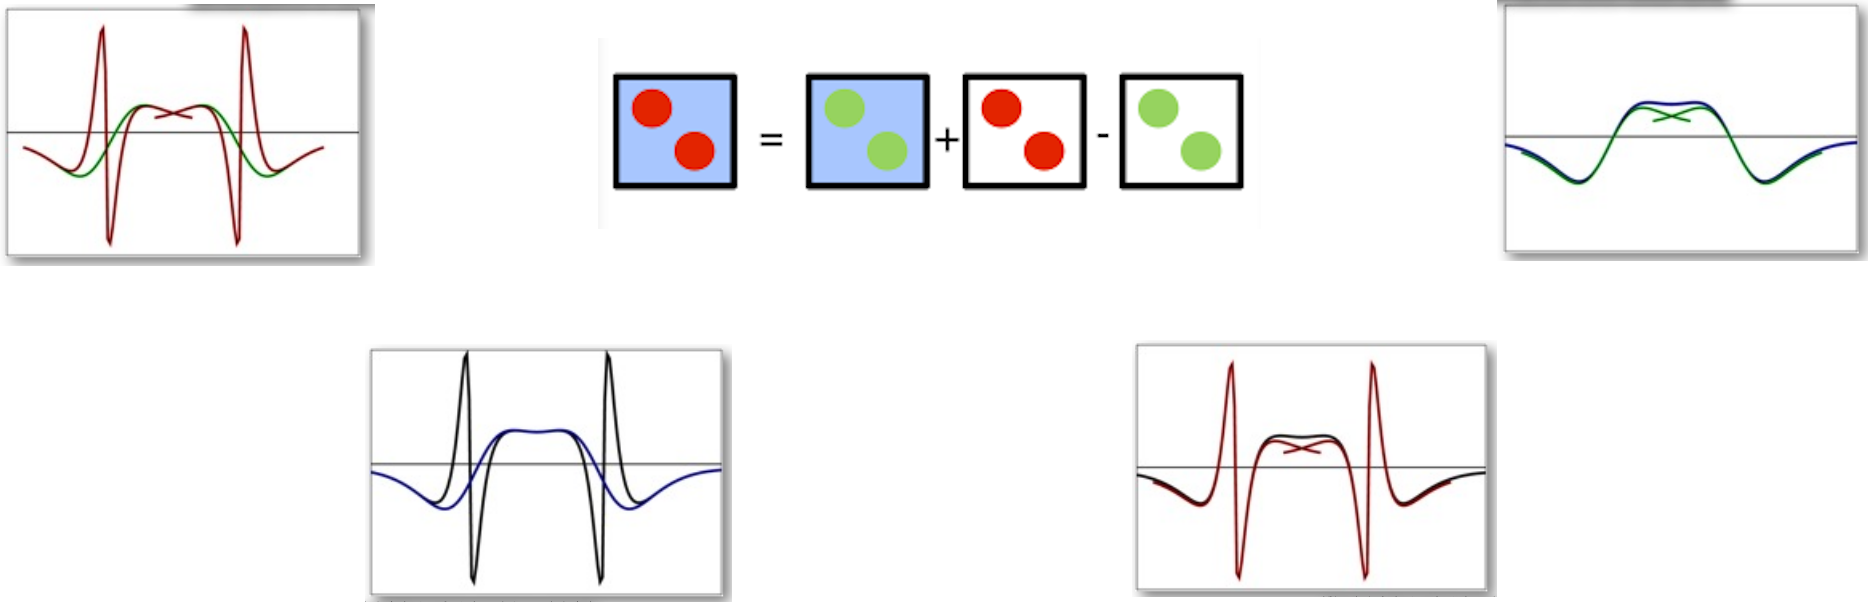
\includegraphics[height=1.7cm, width=2.30cm, viewport=1130 0 1500 265,clip]{Figures/Full_Potential.png}};
	\end{tikzpicture}
}

\frame
{
	\frametitle{固体计算方法总结}
\begin{figure}[h!]
\centering
\vspace*{-0.25in}
%\hspace*{-0.80in}
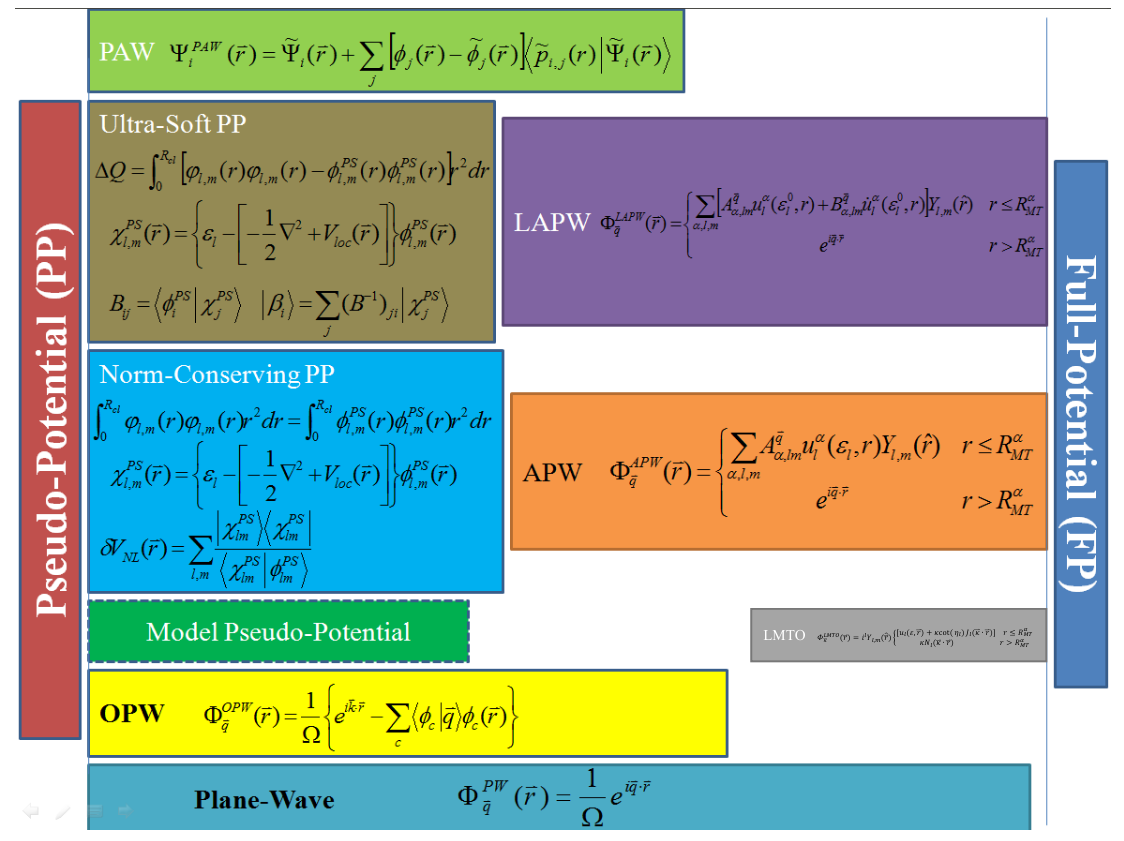
\includegraphics[height=2.80in,width=4.10in,viewport=0 0 1150 850,clip]{Figures/Pseudo-Full_Potential-2.png}
%\caption{\tiny \textrm{Pseudopotential for metallic sodium, based on the empty core model and screened by the Thomas-Fermi dielectric function.}}%(与文献\cite{EPJB33-47_2003}图1对比)
\label{Pseudo-Full_Poential}
\end{figure}
}

\frame
{
	\frametitle{固体计算软件概览}
\begin{figure}[h!]
\centering
\vspace*{-0.05in}
%\hspace*{-0.80in}
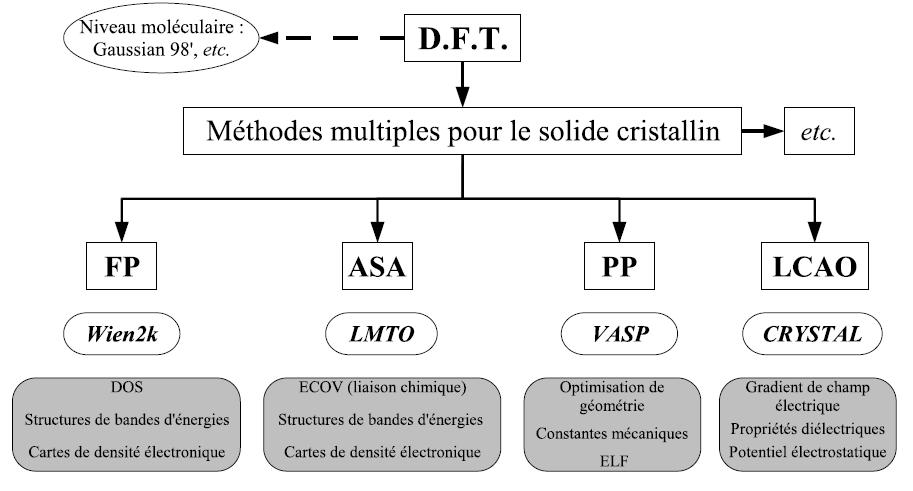
\includegraphics[height=2.30in,width=4.00in,viewport=0 0 920 500,clip]{Figures/DFT-Software.jpg}
%\caption{\tiny \textrm{Pseudopotential for metallic sodium, based on the empty core model and screened by the Thomas-Fermi dielectric function.}}%(与文献\cite{EPJB33-47_2003}图1对比)
\label{Abinitio-Softwares}
\end{figure}
}

%------------------------------------------------------------------------Reference----------------------------------------------------------------------------------------------
		\frame[allowframebreaks]
		{
\begin{thebibliography}{99}
\frametitle{主要参考文献}
{\tiny
	\bibitem{PhysCN40-477_2011}曹则贤, \textit{Secular,equation}, \textit{物理}, \textbf{40} \textrm{(2011), 477}
	\bibitem{Singh}\textrm{D. J. Singh. \textit{Plane Wave, PseudoPotential and the LAPW method} (Kluwer Academic, Boston,USA, 1994)}
	\bibitem{Nemoshkalenko-Antonov}\textrm{V. V. Nemoshkalenko and V. N. Antonov. \textit{Computational Methods in Solid State Physics} (Gordon and Breach Science Publisher, Amsterdam, The Netherlands, 1998)}
	\bibitem{PRB12-3060_1975}\textrm{O. K. Andersen. \textit{Phys. Rev.} B, \textbf{12} (1975), 3060}
	\bibitem{JMP22-2433_1981}\textrm{M. Weiner. \textit{J. Math. Phys.}, \textbf{22} (1981), 2433}
	\bibitem{PRB26-4571_1982}\textrm{M. Weinert, E. Wimmer and A. J. Freeman. \textit{Phys. Rev.} B, \textbf{26} (1982), 4571}
	\bibitem{SSC114-15_2000}\textrm{E. Sj\"ostedt, L. Nordstr\"om and D. J. Singh. \textit{Solid State Commun.}, \textbf{114} (2000), 15}
	\bibitem{Andersen_Book}\textrm{O. K. Andersen. \textit{Computational Methods in Band Theory} (Plenum, New York, USA, 1971)}
}
\end{thebibliography}
\nocite*{}
}
